%!TEX root = Constructive Alignment for Introductory Programming.tex

\chapter{Evaluation of the Teaching and Learning Context} % (fold)
\label{cha:evaluation}

\graphicspath{{Figures/Evaluation/}}

This chapter presents the results from a number of small studies into the effectiveness of the model presented in \cref{cha:approach}. The units analysed match those described in \cref{cha:example_impl}, and they made use of the resources discussed in \cref{cha:supporting}. 

\sref{sec:research_design} describes the action research method, and thematic analysis approach, used in this work and outlines how the ethical issues related to analysing student work were addressed. This is followed by \sref{sec:lessons_learnt_from_action_research} that presents a discussion of the evolution of the model, and the associated resources and assessment criteria, across all iterations of the action research process. \sref{sec:issues_identified_in_student_reflections} and \sref{sec:evaluating_progress_using_burndown_charts} provide the results and discussions from the thematic analysis of student portfolios from two teaching periods. \sref{sec:issues_identified_in_student_reflections} discusses issues that students reported in their reflections, while \sref{sec:evaluating_progress_using_burndown_charts} examines student progress as depicted by the burn down charts included in student portfolios. 

\clearpage
\section{Research Design} % (fold)
\label{sec:research_design}

\subsection{Action Research} % (fold)
\label{sub:action_research}

Due to the practical and applied nature of this research -- with its focus on student learning, and the embedded reflective process -- it was decided to follow a Practical Action Research \cite{Creswell:2008} design based on Mills' \cite{Mills:2010} \emph{dialectic action research spiral}. This model, shown in \fref{fig:mills_spiral}, includes a four step process: (1) identify an area of focus, (2) collect data, (3) analyse and interpret the data, and (4) develop an Action Plan.

\begin{figure}[htbp]
  \centering
  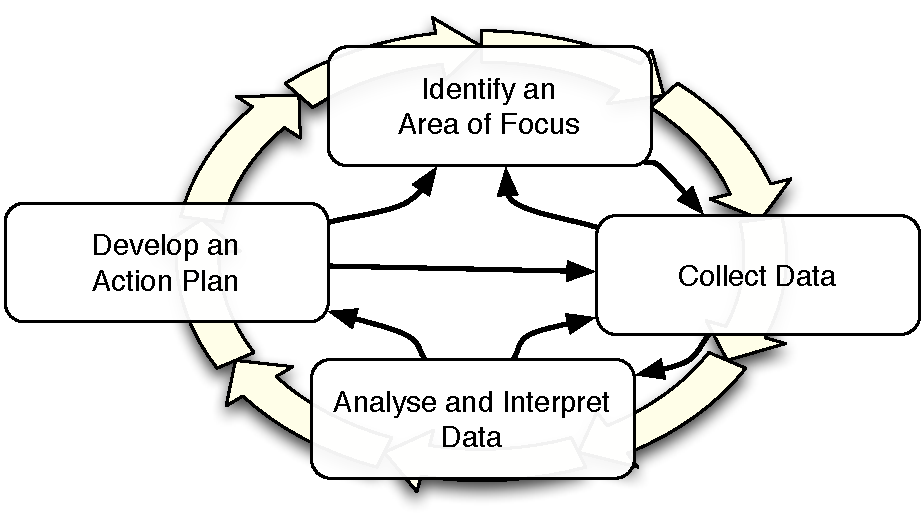
\includegraphics[width=0.7\columnwidth]{MillsSpiral}
  \caption{A visual representation of Mills \cite{Mills:2010} Dialectic Action Research Spiral}
  \label{fig:mills_spiral}
\end{figure}

Iterations in the work presented aligned to teaching periods that included the delivery of one or more of the programming units discussed in \cref{cha:example_impl}. Each iteration included an \emph{action plan} related to implementing the approach from \cref{cha:approach}, which influenced the \emph{focus} for the iteration, the data collected, and the analysis performed.

The overall focus for this research was on the development, application and iterative improvement of the model from \cref{cha:approach}. The iterative nature of the action research process meant that the specific focus in each teaching period addressed relevant aspects of the model, based on its state at that time and feedback from previous iterations. 

Data collection included analysis of student portfolios, student grades, unit documentation and staff reflections, as illustrated in \fref{fig:research_data}. The Unit Outline, prepared prior to the start of the teaching period, documented the intended learning outcomes and assessment criteria around which the unit delivery was focused. Student work from the teaching period was collected and submitted for assessment in student portfolios. Students could opt to make this work available to the action research project using the process outlined in \sref{sub:addressing_ethical_concerns} to address ethical considerations. Reflections from Teaching Staff, Unit Results and Unit Reviews also provided data for the action research project.

\begin{figure}[tbp]
  \centering
  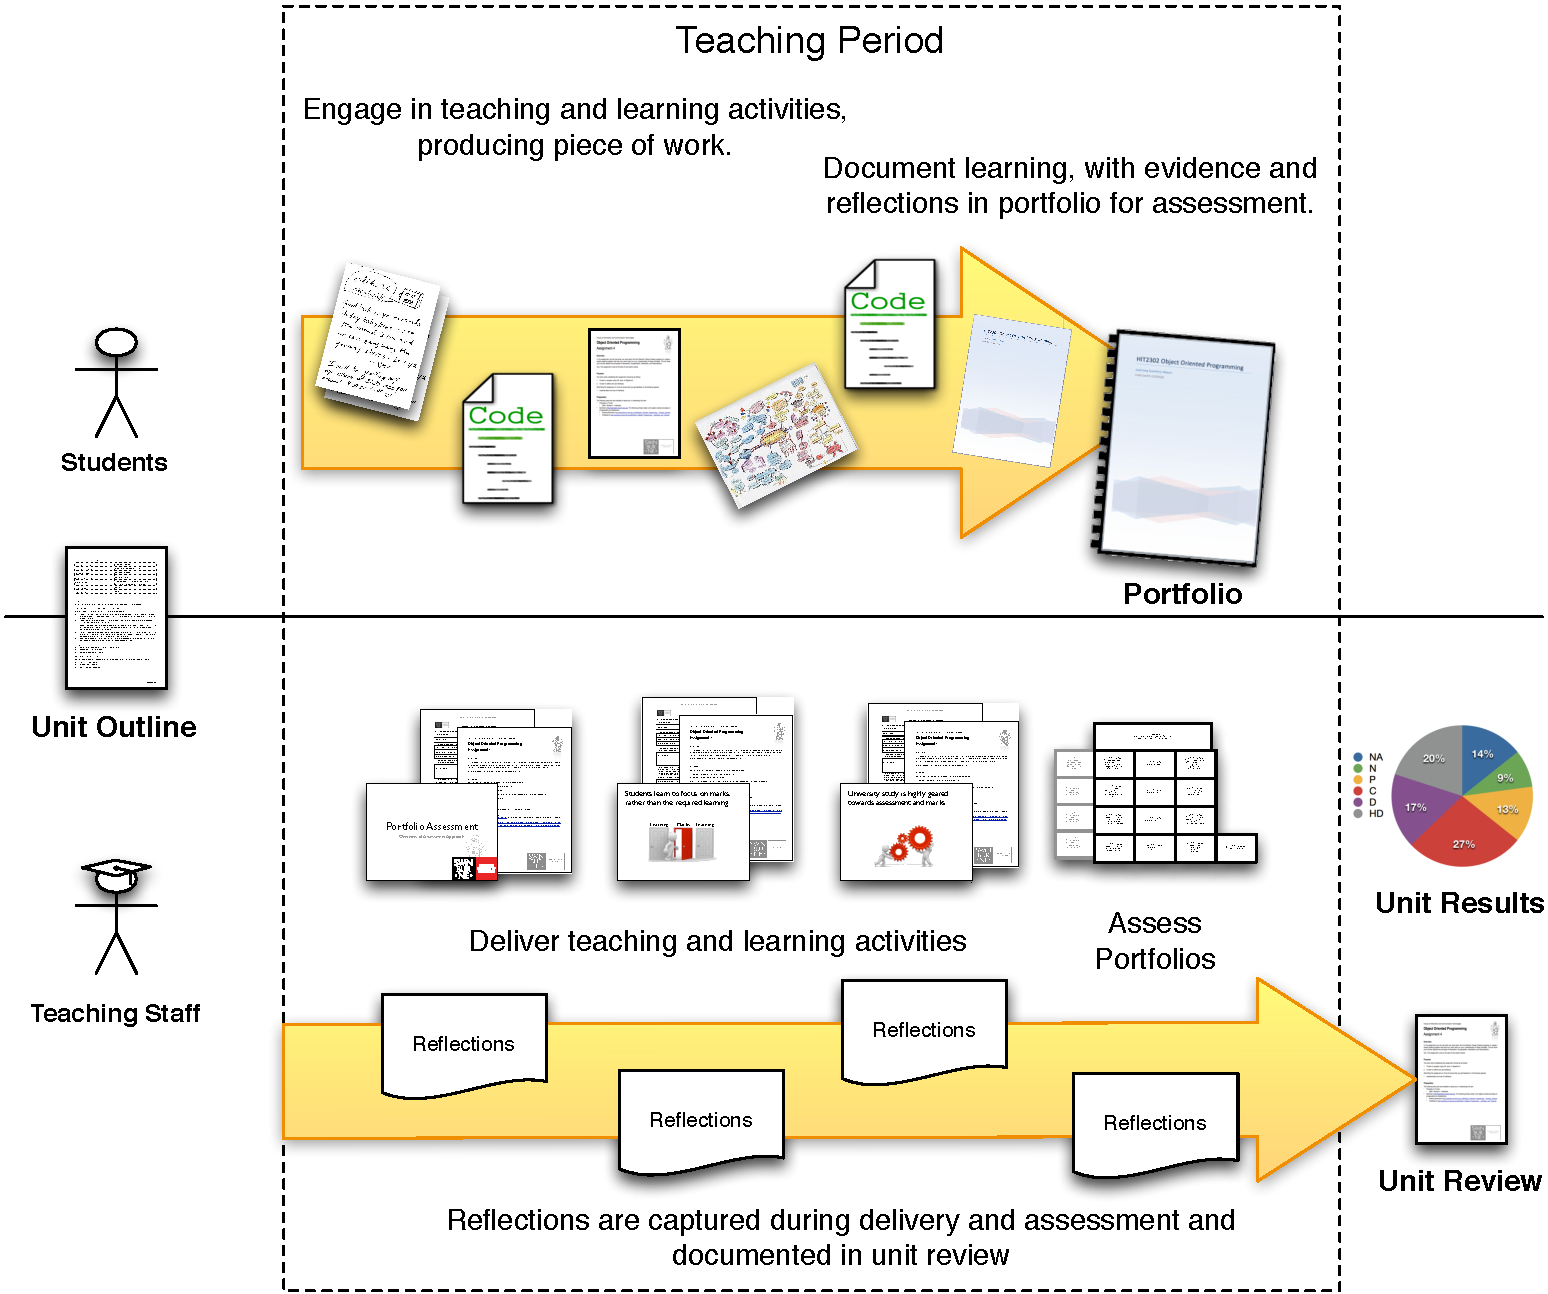
\includegraphics[width=\textwidth]{ResearchData}
  \caption{Various documents used in the data collection for this research}
  \label{fig:research_data}
\end{figure}

Thematic analysis \cite{Braun:2006} was used to examine reflections in student portfolios, which is discussed further in \sref{sub:thematic_analysis}. As the thematic analysis of student portfolios was a time consuming process, it was not performed in all iterations. In teaching periods where a thematic analysis of the portfolios was not performed, the student grades and staff reflections provide insights into the composition of student portfolios.

Unit documentation included the Unit Outline and Unit Review documents. The Unit Outline documented the intended learning outcomes and assessment criteria used in the given teaching period. This document was provided to students prior to the commencement of classes and was an actively used and referred to by both teaching staff and students. At the conclusion of the teaching period, and after results were reported, a Unit Review document was created. This document captured details of student perceptions of the teaching, teaching and learning approach, results, unit management, and any planned changes for future delivery of the unit. These documents were prepared by the Unit Panel, and included input from all teaching staff.

% The learning environment has been found to influence students' approach to learning \cite{Entwistle:1990,Entwistle:1991,Kember:2007}, and perceptions of these environments have been shown to directly, and indirectly, influence learning outcomes \cite{Meyer:1990,Lizzio:2002}. This research attempts to capture this using results from the University's student satisfaction surveys.

Staff reflections indicate the overall and particular qualities exhibited in the student portfolios for a given semester. Staff reflections were captured both during the semester and after portfolios were assessed. These reflections were recorded in personal log book notes, which in most cases were summarised in the Unit Review document.

Student grades provide an indication of how well students performed in the given semester. Together with the staff reflections, results provide some insight into the learning outcomes students achieved -- insights not available by considering students grades alone.

\fref{fig:mills_with_data} illustrates the interactions between the activities in the action research project, and the teaching and learning activities for an individual teaching period. The action research activities, on the left, provided inputs to help refine the model and inform adjustments to the Unit Outline. These activities coincided with the teaching and learning activities associated with defining the intended learning outcomes, and constructing the assessment criteria. 

Interestingly, the Unit Review document provided input into the data collection, while also incorporating inputs from the analysis and interpretation of the data. This was achieved in two phases, initially the teaching staff prepared the unit review incorporating their reflections on the teaching period as well as data from student surveys and unit results. The Unit Review document was then used as part of the action research project, which further analysed the data available. The outputs of this analysis were then added to the Unit Review, to ensure they helped inform subsequent iterations.

\begin{figure}[thbp]
  \centering
  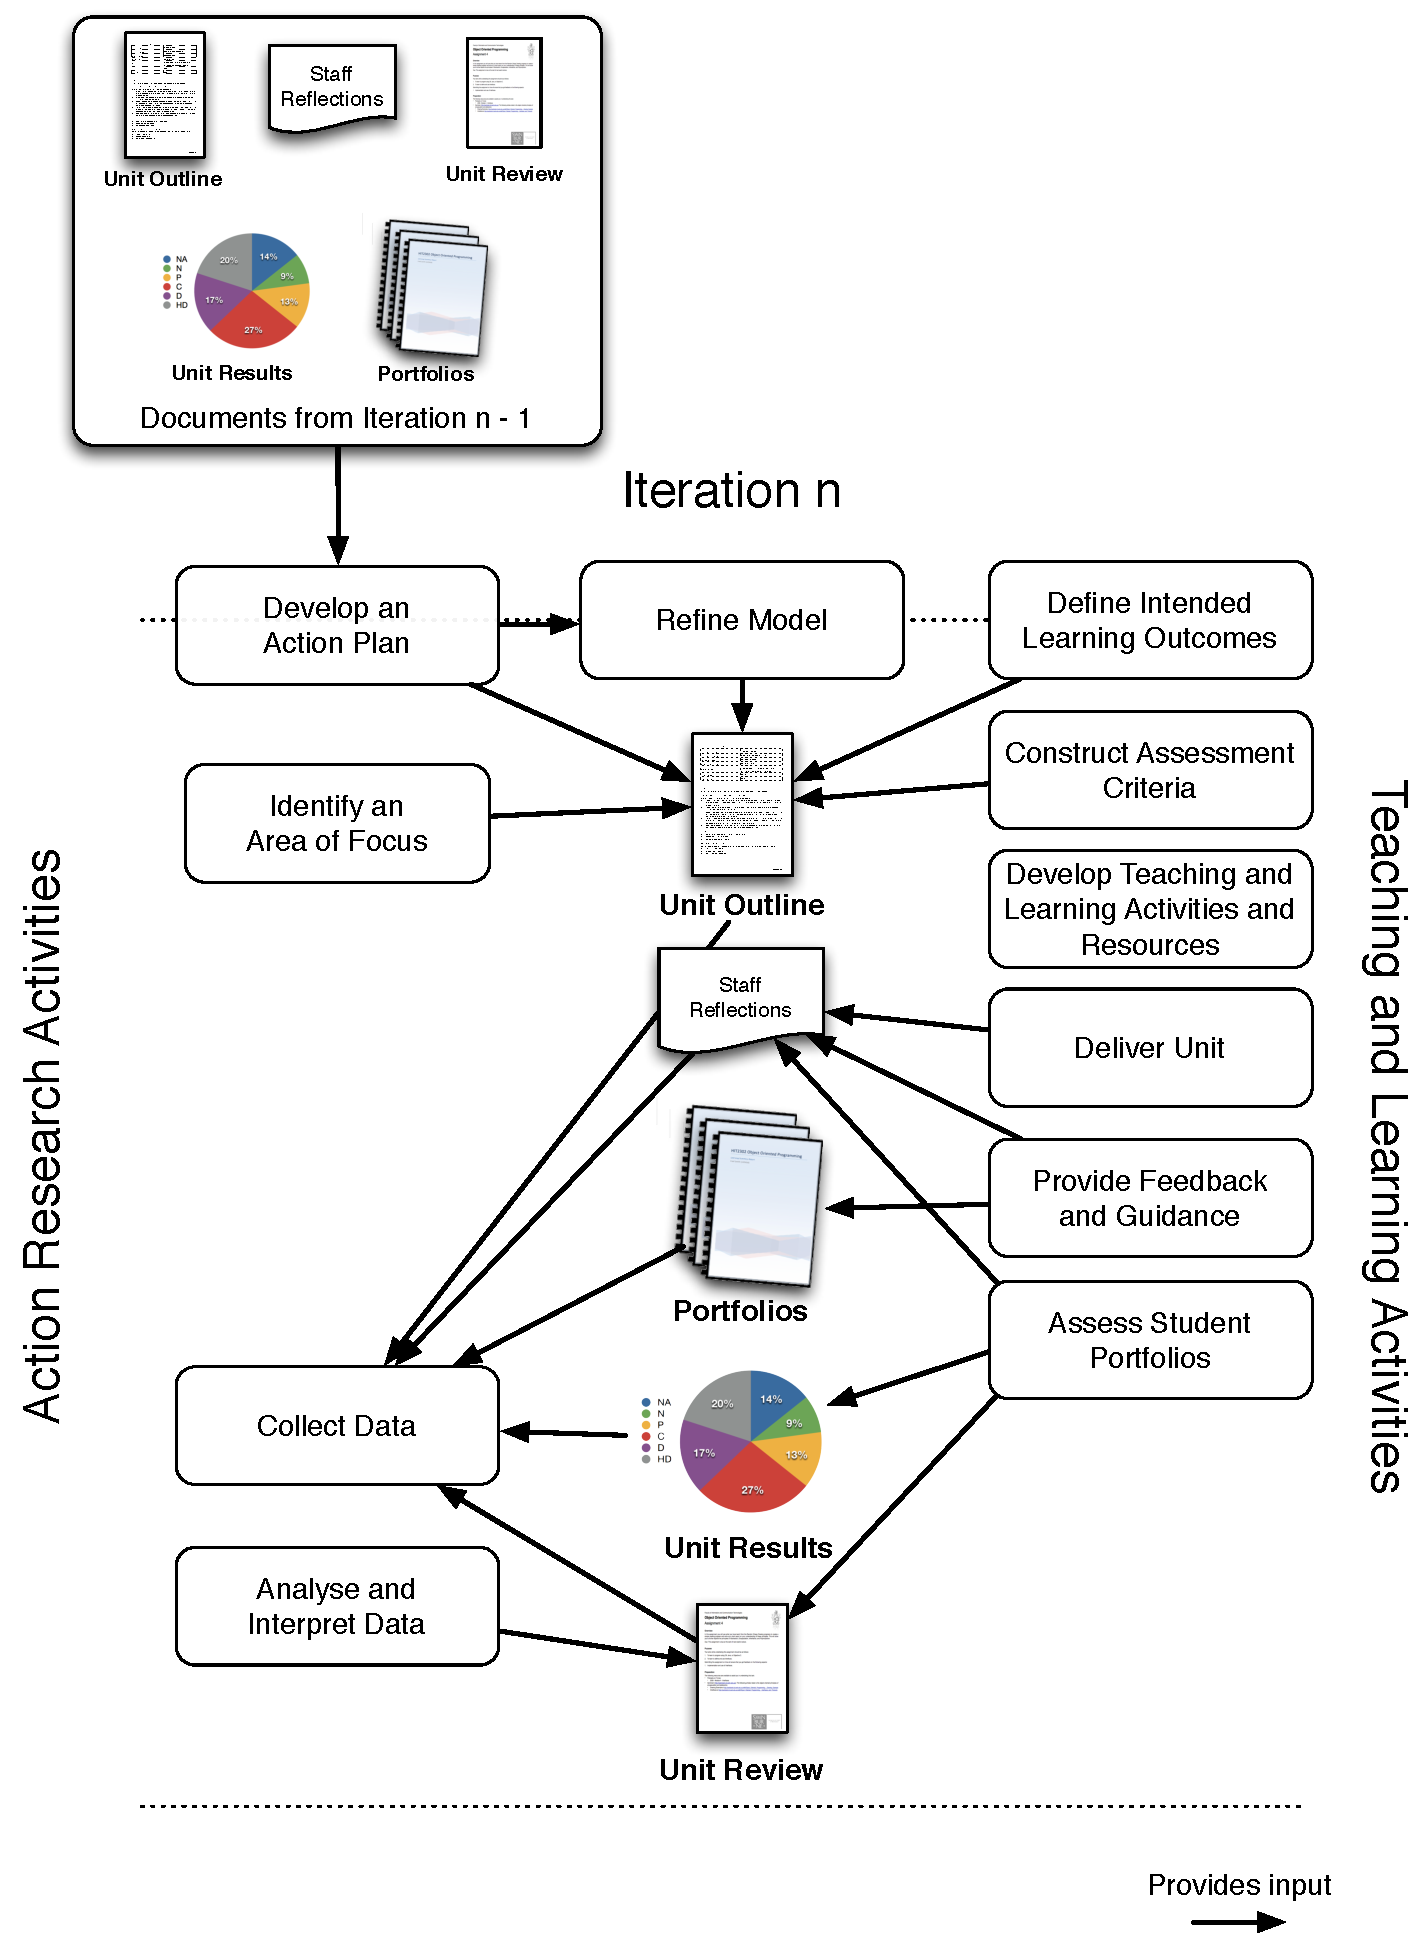
\includegraphics[width=\textwidth]{MillsWithData}
  \caption{Interactions between Action Research Activities and Teaching and Learning Activities, and their input into various documents.}
  \label{fig:mills_with_data}
\end{figure}



% subsection action_research (end)
\clearpage

\subsection{Thematic Analysis of Reflections} % (fold)
\label{sub:thematic_analysis}

Reflections in student portfolios provide a wealth of information. To help identify themes and patterns in the portfolios it was decided to perform a thematic analysis using the process outlined by \citet{Braun:2006}. This process involves six phases, with some terminology\footnote{The term ``code'' has been changed to ``theme'' to avoid confusion relate to the use of this term in computer science.} adapted for clarity:
\begin{enumerate}[noitemsep,nolistsep]
  \item Familiarising yourself with the data
  \item Generating initial themes,
  \item Searching for strong themes
  \item Reviewing themes
  \item Defining and naming themes
  \item Producing the report
\end{enumerate}

In each teaching period where a thematic analysis was performed, familiarity with the data was obtained early in the process with all portfolios being read as part of the unit assessment. At the end of the unit assessment, teaching staff made notes related to general issues, progress, and the overall quality of portfolios. This was part of standard unit delivery procedures, with the resulting reflections being summarised in the Unit Review document as mentioned in \sref{sub:action_research}.

Once the portfolios were made available for this research initial themes were generated by revisiting the reflective component of each portfolio and looking for the qualities under examination. These themes were then documented, and recorded in a spreadsheet. Spreadsheet software was used to collate the themes and record the portfolio details of where these themes had been mentioned, along with any illustrative comments using the students own words.

In phases 3 through 5 the identified themes were broadly grouped together, and then each broad group was examined for sub-themes. All of the themes identified in the examination of student portfolios were maintained in the final categorised results. Themes that did not clearly relate to any of the identified groups were grouped together as a miscellaneous group.

In the reporting of this analysis the raw results are presented, grouped into the identified themes. Illustrative quotes from student reflections are provided to help define the themes.

% subsection thematic_analysis_of_reflections (end)

\clearpage
\subsection{Addressing Ethical Concerns} % (fold)
\label{sub:addressing_ethical_concerns}

In studies related to an educational context, the student-teacher relationship can be a source of potential ethical problems, with perceptions of coercion being the central concern where the research is also involved in teaching the students. Participants in this study were students of the investigators, and so it was important to design an appropriate process whereby students could offer informed consent to participate in the research with no risk of coercion.  

This issue was further complicated as the researchers at times taught both the first and second programming units. For example students could undertake the introductory programming unit in the first half of the year, and the object oriented programming unit in the second half of the year. As most students who completed the first unit progressed to the second unit the following semester, there was the potential for the perception of coercion in this second unit.

An appropriate research protocol was developed, and granted ethical approval from Swinburne's Human Research Ethics Committee. \fref{fig:ethics_process} shows an overview of the protocol approved and used.

\begin{figure}[thb]
  \centering
  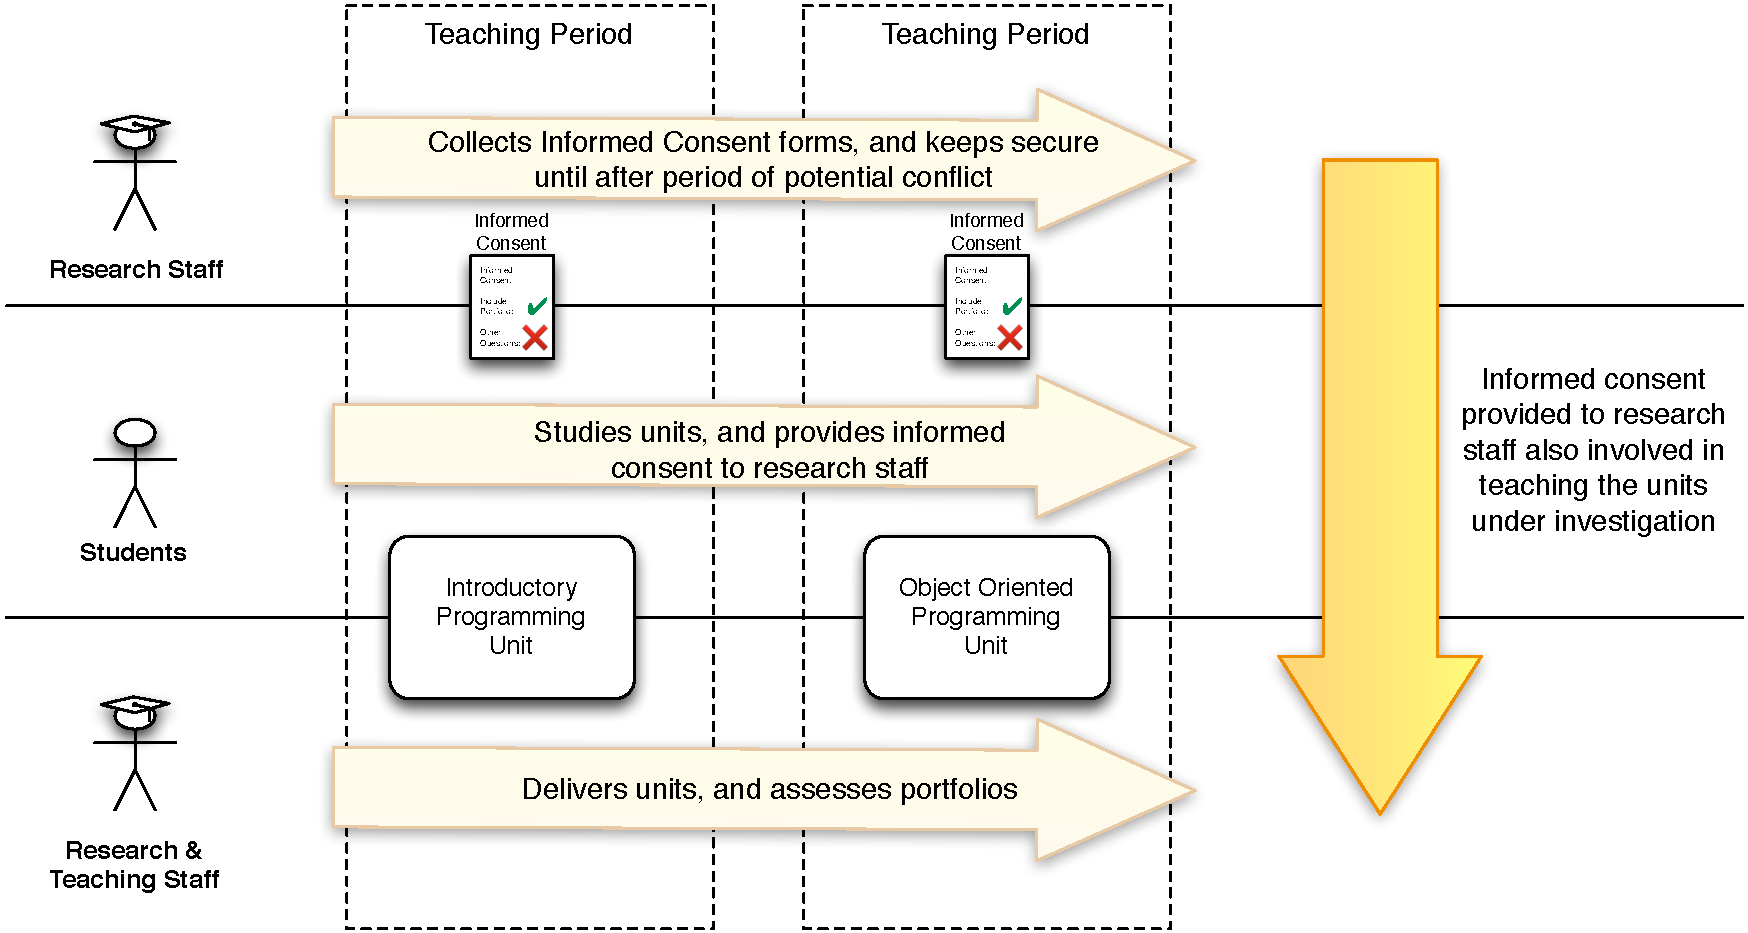
\includegraphics[width=\textwidth]{EthicsProcess}
  \caption{Overview of the protocol used to avoid perceptions of coercion across all units involved in this research}
  \label{fig:ethics_process}
\end{figure}

Students were informed that participation in the research was voluntary, and their participation would in no way influence their results or relationship with the university. Informed consent was then gained using a printed Informed Consent form, which was distributed to students in lectures during each teaching period. Forms were completed by all students, and indicated their willingness to have their work included in the research. All students were required to complete and sign the form, so that it was not be possible to determine those who did, or did not, wish to participate simply by observing those who signed the form.

To avoid issues of coersion in the second programming unit, the Informed Consent forms were withheld from researchers involved in teaching these students until the period of potential influence was deemed to have passed. Until such time, the forms were kept in a sealed envelope in a locked cabinet at Swinburne by the researchers who were not directly involved in teaching of the units.

The period of potential influence was deemed to have passed based on the following:
\begin{itemize}[noitemsep,nolistsep]
	\item For the introductory programming units where the researchers were not involved in teaching a follow on unit, the period of potential influence was deemed to have passed once the results for the introductory programming unit were published.
	\item For the introductory programming units where the researchers were involved in the teaching the follow on unit, the period of potential influence was deemed to have passed once the results for the \emph{second} unit were published.
	\item For the object oriented programming units, the period of potential influence will be deemed to have passed once the results for the unit were published.
\end{itemize}

% subsection addressing_ethical_concerns (end)

% section research_design (end)
\clearpage
\section{Lessons Learnt through Action Research} % (fold)
\label{sec:lessons_learnt_from_action_research}

The action research process was used in the development, application, and evaluation of the model presented in \cref{cha:approach}. A total of nine iterations were completed over a five year period, involving thirteen unit deliveries, with a total of 983 portfolios assessed. This section reports on the development of the model, its guiding principles, the teaching and learning activities and supporting resources.

\subsection{The Units} % (fold)
\label{sub:the_units}

\cref{cha:example_impl} presented details of two example implementations of the model. These examples represent the current status of this research, which evolved iteratively from the delivery of four separate programming units: two introductory programming units, and two object oriented programming units. \tref{tbl:units_iteration} shows the four different programming units, and the iterations in which they were involved. All of the units were taken by undergraduate students early in their degree programme and were convened by the author. 

\begin{table}[htb]
  \footnotesize
  \renewcommand{\arraystretch}{1.3}
  \caption{Units in each iteration.}
  \label{tbl:units_iteration}
  \centering
	\begin{tabular}{l|c|c|c|c|c|c|c|c|c|c}
 		%\hline
		Units \textbackslash{} Iteration & 1 & 2 & 3 & 4 & 5 & 6 & 7 & 8 & 9 & Current \\ \hline
		Introductory Programming (A) & \checkmark & ~ & \checkmark & ~           & \checkmark & \checkmark & ~           & \checkmark & ~ & \checkmark           \\ 
		Introductory Programming (B)    & ~           & ~           & ~           & ~           & ~           & ~           & \checkmark & \checkmark & \checkmark & \checkmark \\ \hline
		Object Oriented Programming (A) & ~           & \checkmark & ~           & \checkmark & ~           & ~           & \checkmark & ~           & \checkmark & \checkmark \\ 
		Object Oriented Programming (B) & ~           & ~           & ~           & ~           & ~           & ~           & ~           & ~           & \checkmark & \checkmark
		%\hline
	\end{tabular}
\end{table}

General details of the four units follow, and any changes to individual iterations are presented in the following sections.

\subsubsection{Introductory Programming (A)} % (fold)
\label{ssub:introductory_programming_a}

Introductory Programming (A) was typically taken by students in their first semester of their degree programme, and introduced them to procedural programming, as outlined in \cref{cha:example_impl}. The intended learning outcomes included: the ability to read and interpret code; write small procedural programs; iteratively use modular and functional decomposition to break problems down; and the ability to apply the principles of structured programming (focusing on blocks of code and using sequence, selection, and repetition). Outcomes were expressed in a programming language neutral manner as the focus of the unit was on the underlying programming concepts.

Introductory programming (A) was taken by students studying a range of degrees. Most students were enrolled in a Bachelor of Science majoring in Computer Science, Professional Software Development or Games Development.

% subsubsection introductory_programming_ (end)

\subsubsection{Object Oriented Programming (A)} % (fold)
\label{ssub:object_oriented_programming_a}

Object Oriented Programming (A) had Introductory Programming (A) as a prerequisite and was predominantly taken by students in their second semester. As outlined in \cref{cha:example_impl}, the intended learning outcomes in this unit required students to: design, develop and test object oriented programs; communicate the underlying principles of abstraction, encapsulation, inheritance and polymorphism; use professional software development tools; and describe factors that influence the quality of an object oriented program. As with Introductory Programming (A), the outcomes were expressed in a language neutral manner and the focus was on underlying concepts.

The student cohort in Object Oriented Programming (A) consisted only of students that had completed Introductory Programming (A).

% subsubsection object_oriented_programming_ (end)

\subsubsection{Introductory Programming (B)} % (fold)
\label{ssub:introductory_programming_b}

Prior to iteration seven this unit was taught using a common textbook style approach with assignments and a final exam. In iteration seven the unit was adapted to a portfolio-based approach, and then combined with Introductory Programming (A) from iteration eight.

Intended learning outcomes for Introductory Programming (B) covered similar topics to Introductory Programming (A) but with specific reference to the C programming language. When this was combined with Introductory Programming (A) in iteration eight, the combined outcomes matched those from \cref{cha:example_impl}, and the focus shifted from language syntax to programming concepts.

The cohort of Introductory Programming (B) included students from a range of degree programmes. This included students studying for a Bachelor of Information and Communication Technology, Bachelor of Engineering and Bachelor of Science (Computer Science and Software Engineering). The unit was included in a number of other degrees as an elective.

% subsubsection introductory_programming_ (end)

\subsubsection{Object Oriented Programming (B)} % (fold)
\label{ssub:object_oriented_programming_b_}

As with Introductory Programming (B), Object Oriented Programming (B) was taught using a specific language (C++), used a textbook style approach, traditional assignments and final exam. This unit covered the same topics as Object Oriented Programming (A), and in iteration nine the two object oriented programming units were combined into a single unit. This combined unit used portfolio assessment and its intended learning outcomes matched those from \cref{cha:example_impl}, and focused on programming concepts and principles. Students continued to enrol in the individual units, but were taught as a single cohort. Students enrolled in Object Oriented Programming (B) were required to include evidence in their portfolios of being able to apply the unit's concepts using the C++ language.

% subsubsection object_oriented_programming_b_ (end)

\subsubsection{Relationship Between Units} % (fold)
\label{ssub:relationship_between_units}

\fref{fig:unit_paths} shows progression paths through these units. The students we broadly classified as being enrolled in a \emph{software development} focused degree took Introductory Programming (A) in the first semester of their first year, and then Object Oriented Programming (A) in the second semester of their first year. Introductory Programming (B) was taken primarily by student enrolled in an Engineering degree, who subsequently took an intermediate programming unit before studying Object Oriented Programming (B). The intermediate programming unit aimed to further develop students' programming knowledge with the C and C++ programming languages, and included a brief introduction to objects in the last few weeks. For the Engineering students, this sequence may be extended over more than three consecutive semesters depending on their degree programme.

\begin{figure}[htbp]
  \centering
  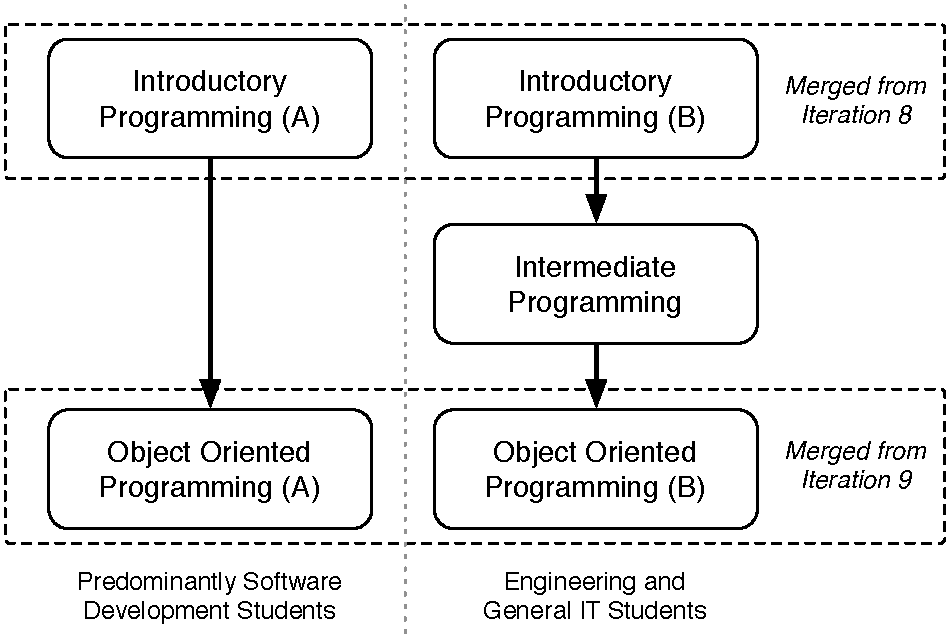
\includegraphics[width=0.62\textwidth]{UnitPaths}
  \caption{Progression pathways through the introductory programming units}
  \label{fig:unit_paths}
\end{figure}

% subsubsection relationship_between_units (end)
% subsection the_units (end)

\subsection{Early Iterations} % (fold)
\label{sub:early_iterations}

\subsubsection{Iteration 1} % (fold)
\label{sub:iteration_1}

\paragraph{Focus} % (fold)

This was our first attempt at constructive alignment and portfolio assessment. This first iteration focused on implementing changes in line with constructivist learning theories and aligned curriculum, namely \pref{itm:construct} and \pref{itm:align} from \cref{cha:guiding_principles}.

\tref{tbl:prin_iter_1} indicates the principles related to this iteration. At this stage the focus was on constructive learning theories (\Pref{itm:construct}) and aligned curriculum (\Pref{itm:align}). Students were actively supported throughout the teaching period (\Pref{itm:support}), the unit focused on concepts associated with a single paradigm (\Pref{itm:paradigm}), and made appropriate use of programming languages used (\Pref{itm:authentic}. Staff were willing to change, but were still progressing toward \pref{itm:agile} as outlined in \cref{cha:guiding_principles}. Similarly, concepts (\Pref{itm:concepts}) were central to the teaching, but lacked the clear focus that developed in later iterations (\Pref{itm:focus}).

\begin{table}[h]
  \centering
  \caption{Principles related to Iteration 1. Focus is indicated by \foci, \done indicates in form presented in \cref{cha:guiding_principles}, \some indicates partially present but neither in planned focus nor in final form.}
  \label{tbl:prin_iter_1}
  \begin{tabular}{l|ccccccccc|ccc}
    Iteration & \Pref{itm:construct} & \Pref{itm:align} & \Pref{itm:formative} & \Pref{itm:focus} & \Pref{itm:expectations} & \Pref{itm:support} & \Pref{itm:theory_y} & \Pref{itm:agile} & \Pref{itm:reflect} & \Pref{itm:paradigm} & \Pref{itm:concepts} & \Pref{itm:authentic} \\
    \hline
    %               P1      P2      P3      P4      P5      P6      P7      P8      P9     P10     P11     P12
    Iteration 1 & \foci & \foci & \none & \some & \none & \done & \none & \some & \none & \done & \some & \done \\
  \end{tabular}
\end{table}


\paragraph{Action Plan} % (fold)

The approach used was an iterative step toward the general model presented in \cref{cha:approach}. Students were required to complete six assignments and six tests, with the \emph{option} to include a portfolio. The aim of the assessment strategy was for students to demonstrate their understanding of core concepts in the assignments and tests, with the portfolio used to determine student ability in the higher grade brackets. Weights were applied to each of the assessment items and these were added together to calculate the final grade.

In terms of the model from \cref{cha:approach}, this iteration lacked many of the aspects defined. Intended learning outcomes had been defined, there were some assessment criteria (though they lacked the clarity of later iterations) teaching and learning activities were presented to students with lectures including interactive components, and students did present a portfolio of work for assessment. The major difference was the lacked of the iterative formative feedback process. The dynamic from this iteration was more consistent with ``standard'' teaching and learning environments teaching staff had experienced before implementing constructive alignment, with the portfolio representing yet another assignment.

Key differences from the portfolio model presented in \cref{cha:approach}:
\begin{itemize}[noitemsep,nolistsep]
  \item The unit included a total of eleven intended learning outcomes, each making use of active verbs and relating to specific parts of the unit.
  \item It used multiple assignments (six) over the semester.
  \item It included tests that were marked and contributed to the final grade.
  \item Submission of a portfolio was optional.  All students who submitted a portfolio were interviewed.
\end{itemize}

Similarities with later portfolio iterations included:
\begin{itemize}[noitemsep,nolistsep]
  \item It included qualitative criteria for each grade, though these were described in general terms.
  \item Students included a self assessment against the criteria.
\end{itemize}

Key differences from the introductory programming unit described in \cref{cha:example_impl} included the following:
\begin{itemize}[noitemsep,nolistsep]
	\item Focus was on programming concepts, but there was some crossover of topics in the early material.
	\item The teaching and learning activities made limited use of SwinGame.
	\item Procedures were introduced later (SwinGame was not used in the early parts of the teaching period). 
	\item Students were only briefly introduced to the C programming language at the end of the unit.
	\item None of the supporting tools from \cref{cha:supporting} had been developed at this stage.
	\item Lecture slides closely followed the ``Beyond Bullet Points'' approach \cite{Atkinson:2007}, and included extensive notes on each slide.
	\item An earlier edition of the Pascal Language Reference \cite{FPC:2013lang} was used as the unit text.
\end{itemize}

\paragraph{Data} % (fold)

Unit results across all iterations are shown in \tref{tbl:unit_results}, which lists the number of students receiving each grade over the nine iterations. Grades include those students who enrolled but did not submit a portfolio (NA) those who failed (N) and those who received Pass (P) Credit (C) Distinction (D) and High Distinction (HD) result. The results for Iteration 1 are shown in \fref{fig:iterations_1_2}. In this iteration a large percentage of students managed to receive an HD grade.

\begin{table}[p]
  \footnotesize
  \renewcommand{\arraystretch}{1.3}
  \caption{Unit Results Across Iterations 1 to 9}
  \label{tbl:unit_results}
  \centering
    \begin{tabular}{l|l|c|c|c|c|c|c}
        Iter. & Unit    & NA & N  & P  & C  & D  & HD \\ \hline
        1         & Introductory Programming (A)  & 3  & 1  & 4  & 5  & 6  & 11 \\ \hline
        2         & Object Oriented Programming (A) & 19 & 7  & 14 & 19 & 13 & 11 \\ \hline
        3         & Introductory Programming (A)  & 9  & 1  & 2  & 9  & 6  & 9  \\ \hline
        4         & Object Oriented Programming (A) & 4  & 7  & 3  & 17 & 6  & 5  \\ \hline
        5         & Introductory Programming (A)  & 10 & 6  & 9  & 19 & 12 & 14 \\ \hline
        6         & Introductory Programming (A)  & 14 & 3  & 28 & 20 & 14 & 5  \\ \hline
        7         & Introductory Programming (B)  & 42 & 12 & 56 & 47 & 22 & 7  \\ 
        ~         & Object Oriented Programming (A) & 5  & 8  & 18 & 10 & 8  & 9  \\ \hline
        8         & Introductory Programming (A)  & 11 & 5  & 20 & 21 & 17 & 14 \\ 
        ~         & Introductory Programming (B)  & 39 & 47 & 84 & 36 & 20 & 9  \\ \hline
        9         & Introductory Programming (B)  & 61 & 4  & 78 & 24 & 25 & 7  \\ 
        ~         & Object Oriented Programming (A) & 14 & 0  & 25 & 6  & 14 & 7  \\ 
        ~         & Object Oriented Programming (B) & 7  & 0  & 25 & 5  & 3  & 4  
    \end{tabular}
\end{table}

\begin{figure}[p]
  \centering
  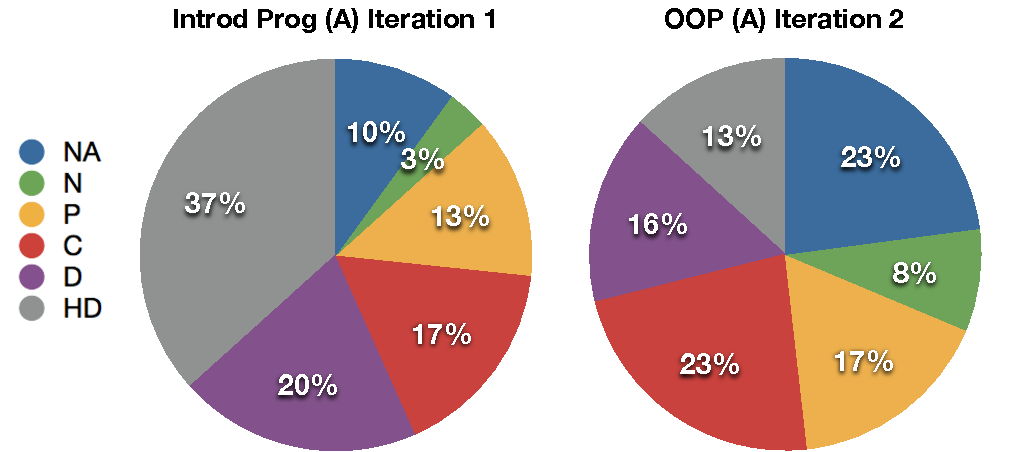
\includegraphics[width=0.8\columnwidth]{Iterations1_2}
  \caption{Result distributions from Iterations 1 and 2, note in particular the shift in the number of High Distinctions.}
  \label{fig:iterations_1_2}
\end{figure}

\paragraph{Reflections and Analysis} % (fold)
\label{ssub:analysis}

Use of portfolios was limited in this iteration, with positive and negative results. Positive aspects of the unit delivery included the improved confidence of staff in the potential for using portfolio assessment in units related to software development. Overall, it was felt that portfolio assessment offered great potential, but that this iteration had not managed to create a suitable environment in which these benefits could be realised.

The two main issues were the weakness of the expressed assessment criteria and the combining of results from the assignments and tests. Together, these issues resulted in many students receiving a higher grade than staff felt was appropriate given the outcomes demonstrated in student portfolios. This is supported by the high portion of students with HD grades when informally compared with other unit results.

Staff reflections included several interesting aspects related to the assessment in this iteration:
\begin{itemize}[noitemsep,nolistsep]
  \item There were too many intended learning outcomes. This had made it difficult for staff to clearly communicate how teaching and learning activities related to the outcomes. Students had also found it difficult to relate their portfolio pieces back to the intended learning outcomes.
  \item Criteria were difficult to apply, being weakly defined, and student interpretations tended to weaken the criteria further in their self assessment.
  \item Significant effort had been put into creating ``Beyond Bullet Point'' slides and associated notes, which had been useful in terms of delivery but restricted opportunities to adapt the material.
  \item Assessing the portfolios was very time consuming due to the loosely defined criteria. Staff needed to ``extract'' value from the portfolios, rather than the emphasis being on students demonstrating understanding.
  \item The time consuming nature of the portfolio assessment meant that teaching staff did not feel the approach could scale to larger class sizes.
  \item Staff felt confident that a portfolio of work could provide a suitable means of assessing student outcomes in technical units, addressing a key concern at the time.
  \item Core assignments and tests:
  \begin{itemize}[noitemsep,nolistsep]
    \item Covered the minimum expectations for the intended learning outcomes.
    \item Received high marks, which only indicated basic coverage of the intended learning outcomes. 
  \end{itemize}
  \item Students with weak portfolios, showing shallow coverage of the intended learning outcomes, were still able to receive high grades indicating the assessment strategy was poor.
\end{itemize}


\paragraph{Development of Principles} % (fold)

The first experience of delivering a portfolio assessed unit had been informed by examining the principles of constructive alignment, and the experience provided a number of insights that helped form the principles stated in \cref{cha:guiding_principles}. These included:

\begin{itemize}[noitemsep,nolistsep]
	\item Constructive learning theories (\Pref{itm:construct}) and aligned curriculum (\Pref{itm:align}) had been at the centre of this experience. However, the utility of both had been hampered by the large number of intended learning outcomes. This guided the importance of having a small number of more highly targeted outcomes.
	\item The portfolios had been able to capture student outcomes, but results had been impacted by the use of weighted assessment used to motivate students during the semester. While alternative schemes, or weightings, could have been developed, it was felt these incentives were not required and a greater use of formative feedback would be of greater benefit to students. This emphasis on formative feedback evolved into \pref{itm:formative} and influenced a change from a soft Theory X to Theory Y (\Pref{itm:theory_y}) perspective.
	\item Teaching staff were \emph{willing to change}, and wanted to be able to adjust teaching material in response to student issues. However, the significant effort that had gone into the develop of the ``Beyond Bullet Points'' lecture slides had created a resistance to change. This conflict started a change in attitude that resulted in the definition of \pref{itm:agile}; the aim to be both \emph{agile} and \emph{willing to change}.
\end{itemize}

% paragraph development_of_principles (end)

% subsection iteration_1 (end)

\subsubsection{Iteration 2} % (fold)
\label{sub:iteration_2}

\paragraph{Focus} % (fold)

Iteration 2 included the delivery of Object Oriented Programming (A), and aimed to address several of the main concerns from Iteration 1 by having \emph{fewer intended learning outcomes} around which everything would be based, assessing each student's outcomes as a whole with \emph{100\% portfolio assessment}, and using \emph{specific assessment criteria} to express what was expected for each grade. In addition to this, the unit material was separated into teaching and learning \emph{activities} and teaching and learning \emph{resources}, in an effort to enable greater flexibility with future changes.

\tref{tbl:prin_iter_2} shows the principles related to this iteration, highlighting the additional focus on frequent formative feedback (\Pref{itm:formative}), adoption of Theory-Y perspectives on motivation (\Pref{itm:theory_y}), and on means of effectively managing teaching and learning activities and resources (\Pref{itm:agile}).

\begin{table}[h]
  \centering
  \caption{Principles related to Iteration 2. Focus indicated by \foci, present indicated by \done, partially present indicated by \some.}
  \label{tbl:prin_iter_2}
  \begin{tabular}{l|ccccccccc|ccc}
    Iteration & \Pref{itm:construct} & \Pref{itm:align} & \Pref{itm:formative} & \Pref{itm:focus} & \Pref{itm:expectations} & \Pref{itm:support} & \Pref{itm:theory_y} & \Pref{itm:agile} & \Pref{itm:reflect} & \Pref{itm:paradigm} & \Pref{itm:concepts} & \Pref{itm:authentic} \\
    \hline
    %               P1      P2      P3      P4      P5      P6      P7      P8      P9     P10     P11     P12
    Iteration 2 & \foci & \foci & \foci & \some & \none & \done & \foci & \foci & \none & \done & \some & \done \\
  \end{tabular}
\end{table}


\paragraph{Action Plan} % (fold)
\label{ssub:develop_an_action_plan2}

The transition from assignments \emph{plus} portfolio, to 100\% portfolio assessment meant that this iteration did include most aspects of the model described in \cref{cha:approach}. Most notably, the iterative feedback process was initiated, and students were actively encouraged to develop pieces for their portfolios throughout the teaching period. Where the model did differ was in how the various activities were guided, as result of the absence of \pref{itm:expectations} and the overly zealous application of constructive learning theories (\Pref{itm:construct}).

In this iteration the following aspects of our model were included:
\begin{itemize}[noitemsep,nolistsep]
  \item The number of intended learning outcomes was reduced from eleven to five, reducing redundancy and providing a clearer focus (\pref{itm:focus}).
  \item Assessment criteria were developed for each grade using the different levels from the SOLO taxonomy \cite{Biggs:1982}. This was presented in a format similar to that shown in \fref{fig:assessment_criteria}, though some details differed.
  \item Feedback was provided to students using weekly formative assessments and tests.
  \item Notes previously embedded in slides were shifted to a single document and distributed to students as a PDF.
\end{itemize}

The following aspects differed from Iteration 1:
\begin{itemize}[noitemsep,nolistsep]
  \item Each intended learning outcome had criteria for meeting it to differing standards: Marginal, Adequate, Good, and Excellent.
  \item A Credit grade required three intended learning outcomes to be addressed at an \emph{Adequate} standard, Distinction required two at a \emph{Good} standard (with all other adequate) and High Distinction required two \emph{Excellent} and all others \emph{Good}.
  \item A flipped classroom model \cite{Baker:2000,Lage:2000} was adopted: student were provided with online videos covering the typical weekly lecture material and class room activities were predominantly interactive.
\end{itemize}

Key differences from the final version of the object oriented programming unit described in \cref{cha:example_impl} include the following:
\begin{itemize}[noitemsep,nolistsep]
	\item A greater emphasis was placed on constructive learning theories, and a shift toward discovery learning. Concepts were presented using the video podcasts, and lecture activities included a greater emphasis on group discussions.
	\item Lectures used a number of interactive quizzes; questions were typically taken, then discussed in small groups, and retaken before a wider group discussion on any changes in understanding.
  \item While multiple languages were used, and students could only choose between the Java and C\# programming languages.
	\item Laboratory exercises also had less guidance, and students explored their chosen language and how it could be used to implement object oriented programs.
	\item SwinGame was introduced early in the teaching period to enable students to visualise object interactions through the creation of a drawing program.
\end{itemize}

% subsubsection develop_an_action_plan (end)

\paragraph{Data} % (fold)
\label{ssub:data2}

\fref{fig:iterations_1_2} shows the result distributions for Object Oriented Programming (A) in Iteration 2. The number of High Distinction results was closer to expectations, though the low pass rate was a cause for concern. 

\paragraph{Reflections and Analysis} % (fold)
\label{ssub:staff_reflections_and_analysis2}

Key staff reflections included:
\begin{itemize}[noitemsep,nolistsep]
  \item The shift to formative feedback had been challenging, with a great deal of anxiety for teaching staff about whether students would engage in the weekly tasks when they had not been allocated marks. 
  \item Interviewing all students provided staff with high confidence that students had completed the work themselves, but meant that portfolio assessment was very time consuming.
  \item The general structure of the assessment criteria was suitable, but there was a disconnect in student perception of the required standard: the interpretation of ``good'' was significantly different between staff and students. Students felt that Good equated to having completed the work, whereas staff viewed this as the required standard for Adequate and Good required the work to be of a higher standard.
  \item The quality of work included in student portfolios was of a weaker standard than desired across all grades.
  \item Most students did not appear to benefit from the classroom flip, with few preparing adequately for the classroom discussions.
  \item It was felt that many students ``coasted'' along, and did not genuinely attempt the planned activities.
  \item Progress on understanding weekly topics was very slow, with the lack of guidance resulting in students not making the best use of their time.
  \item Separation of teaching and learning activities and resources had enabled a greater freedom in creating the interactive lecture, and the resources could be reused for future unit deliveries.
\end{itemize}

Staff felt that most of the issues from the semester could be attributed to the shift toward non-productive ``discovery learning'' \cite{Anderson:1998}. In our effort to implement constructive learning theories we had reduced the amount of guided learning activities, and student productivity appeared to have been adversely affected.

It was still felt that portfolio assessment could be beneficial but that, again, we had failed to realise any significant benefits. In many ways the results from this teaching period, in terms of student learning outcomes, had felt like a backward step.

\paragraph{Development of Principles} % (fold)

The teaching and learning environment created in Iteration 2 had been informed by the constructive learning theories, and a trusting Theory Y environment. At the end of this iteration it was felt that the Theory Y attitude was still appropriate, but that the overly zealous application of constructive learning theories had meant students were unable to appropriately apply themselves. The lack of guidance had resulted in many students spending too much time working out \emph{what} it was they needed to learn, and not enough time \emph{applying} the concepts related to object oriented programming to actually \emph{construct} the required knowledge.

This experience influenced a number of the principles stated in \cref{cha:guiding_principles}. 

\begin{itemize}[noitemsep,nolistsep]
	\item Constructive learning theories, central to \pref{itm:construct}, were tempered to include stronger guidance along with the focus on the central role of the learner in constructing their own knowledge. 
	\item We needed to more clearly communicate our high expectations of students (\Pref{itm:expectations}). In this iteration many students did not seem to be aware of what had been expected of them.
	\item The shallow responses and evidence in student portfolios also indicated the need to focus on depth of understanding (\Pref{itm:focus}).
\end{itemize}

% subsubsection iteration_2 (end)

% subsection early_iterations (end)
\clearpage
\subsection{As the Model Stabilised} % (fold)
\label{sub:as_the_model_stabilised}

Experiences from iterations 1 and 2 had hinted at the potential for portfolio assessment, but the implementation had been unsuccessful. The changes to the model at the end of Iteration 2 resulted in a more successful application of portfolio assessment, and Iterations 3 to 6 all applied the model in a similar way. 

\subsubsection{Iterations 3 to 6} % (fold)
\label{ssub:iterations_3_to_6}

\paragraph{Focus} % (fold)
\label{ssub:focus_3_6}

The focus of Iterations 3 to 6 was on both extended how we taught the units, and developing resources to support what we taught. In relation to how we taught, the focus was on the development of assessment criteria, with the aim to ensure these were clear for both staff and students, and could be applied efficiently to assess student outcomes. At the same time, each iteration worked on extending the resources available to support what and how we taught.

\tref{tbl:prin_iter_3_6} indicates the principles in focus for iterations 3 to 6. Iteration 3 was the first iteration in which all of the principles were present in some form, with most being actively incorporated to address limitations identified in Iteration 2. After this iteration the majority of the principles were in place, and subsequent the focus in subsequent iterations was on improving the incorporation of these principles. Iteration 5 marks the next change, with the incorporation of the hurdle tests and template for the learning summary report. 

\begin{table}[h]
  \centering
  \caption{Principles related to Iterations 3 to 6. This uses the same symbols as in \tref{tbl:prin_iter_1} and \tref{tbl:prin_iter_2}: focus \foci, present \done, partially present \some.}
  \label{tbl:prin_iter_3_6}
  \begin{tabular}{l|ccccccccc|ccc}
    Iteration & \Pref{itm:construct} & \Pref{itm:align} & \Pref{itm:formative} & \Pref{itm:focus} & \Pref{itm:expectations} & \Pref{itm:support} & \Pref{itm:theory_y} & \Pref{itm:agile} & \Pref{itm:reflect} & \Pref{itm:paradigm} & \Pref{itm:concepts} & \Pref{itm:authentic} \\
    \hline
    %               P1      P2      P3      P4      P5      P6      P7      P8      P9     P10     P11     P12
    Iteration 3 & \foci & \foci & \foci & \foci & \foci & \done & \foci & \foci & \foci & \done & \some & \done \\
    Iteration 4 & \done & \done & \some & \foci & \some & \done & \some & \some & \some & \done & \some & \done \\
    Iteration 5 & \done & \done & \some & \some & \some & \done & \foci & \foci & \foci & \done & \some & \done \\
    Iteration 6 & \done & \done & \some & \some & \some & \done & \done & \done & \done & \done & \some & \done \\
  \end{tabular}
\end{table}

In terms of the model described in \cref{cha:approach}, Iterations 3 onward incorporated all aspects. Each iteration provided greater insights into how to successfully deliver units in this approach, and the related guidelines were developed from the changes made from Iteration 3 to Iteration 9.


% subsubsection focus (end)

\paragraph{Action Plan} % (fold)
\label{ssub:plan_3_6}

Assessment criteria in each iteration adopted the changes from prior iterations, and made improvements in wording to better capture staff intentions and expectations for each grade criteria. An example of the overall assessment criteria is shown in \fref{fig:i6_assessment_criteria}, and details of the assessment criteria related to an individual intended learning outcome is shown in \fref{fig:i6_assessment_criteria_detail}.

Specific changes included: 
\begin{enumerate}[noitemsep,nolistsep]
  \item Iteration 3: Changes in this iteration aimed to address the poor outcomes from Iteration 2 by providing students with additional guidance, and communicating our high expectation of their outcomes (\Pref{itm:expectations}). 
  \begin{itemize}[noitemsep,nolistsep]
    \item The flipped classroom idea was dropped, with videos now being used to support classroom activity. This aimed to use a more moderate form of constructive learning theories inline with the ideas communicated in \pref{itm:construct}.
    \item Adjusted the main category descriptors to: Adequate, Good, Outstanding, and Exemplary. Students had interpreted ``good'' to a much weaker standard than staff, shifting this down a category helped better indicate the desired standards. 
    \item A specific reflective report was added as required piece in student portfolios. The report included a self assessment, in which the student aligned the pieces they submitted to the intended learning outcomes, and general reflections (\pref{itm:reflect}). This aimed to help students identify how their work aligned with learning outcomes, while also assisting staff in assessing student portfolios.
  \end{itemize}
  \item Iteration 4: This iteration aimed to reduce the amount of work students needed to do in order to get higher grades, thereby enabling students to focus on building depth of knowledge. (\Pref{itm:focus})
  \begin{itemize}[noitemsep,nolistsep]
    \item Reduced the number of items expected for each grade: Credit required one Good, Distinction one Good another Outstanding, and High Distinction required one Good another Outstanding and a further one at Exemplary.
  \end{itemize}
  \item Iteration 5: The success of iteration 4 meant that iteration 5 made only slight adjustments aimed at improving productivity.
  \begin{itemize}[noitemsep,nolistsep]
    \item Pass and Credit students were no longer interviewed. Interviews had been used to assess all students up to this point, but the use of common tasks by all Pass and Credit students meant that staff felt the model could be adjusted to use hurdle tests and no longer require an interview for students aiming for Pass and Credit. (\Pref{itm:agile})
    \item Tests became a hurdle requirement, and had to be completed to a satisfactory standard for students to be eligible to pass the unit. Students who did not pass the test first time, could sit a second test at a later date. (\Pref{itm:formative})
  \end{itemize}
  \item Iteration 6: Staff reflections from Iteration 5 indicated the Distinction and High Distinction grade criteria could be better organised as most students favoured only one or two of the intended learning outcomes. It was decided to rethink the criteria to better define what each grade category meant.
  \begin{itemize}[noitemsep,nolistsep]
  	\item Short reports that discussed aspects related to each intended learning outcome were required to meet the \emph{Good} standard.
    \item To meet the \emph{Outstanding} standard for an intended learning outcome, students were required to develop a program of their own design and relate this to intended learning outcomes.
    \item Meeting the \emph{Exemplary} standard required a research report related to the intended learning outcome. 
  \end{itemize}
\end{enumerate}

\begin{figure}[p]
	\centering
	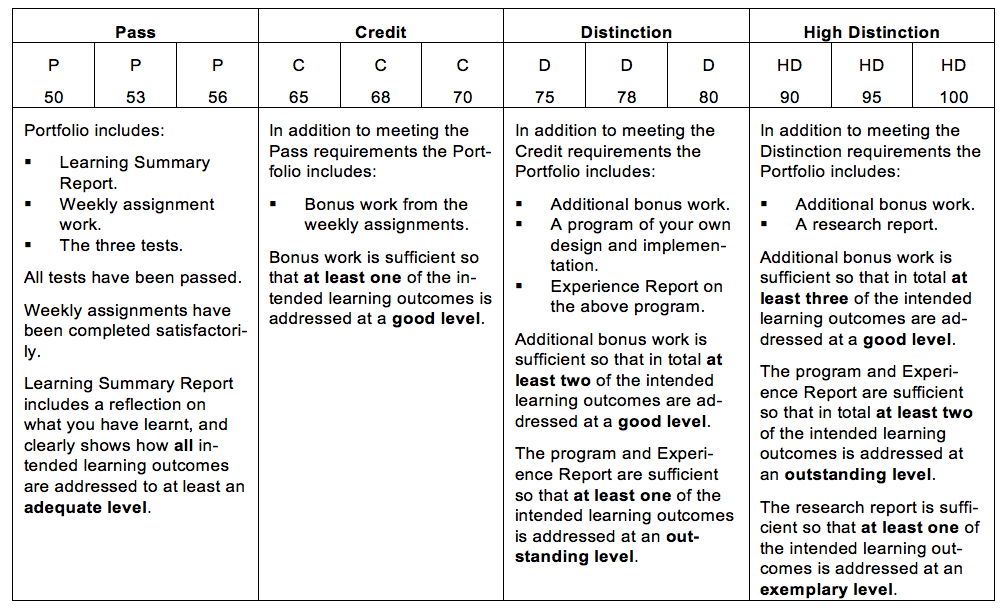
\includegraphics[width=0.95\textwidth]{AssessmentCriteria}
	\caption{Overview assessment criteria provided to students in the unit outline of Introductory Programming (A) in Iteration 6.}
	\label{fig:i6_assessment_criteria}
\end{figure}

\begin{figure}[p]
	\centering
	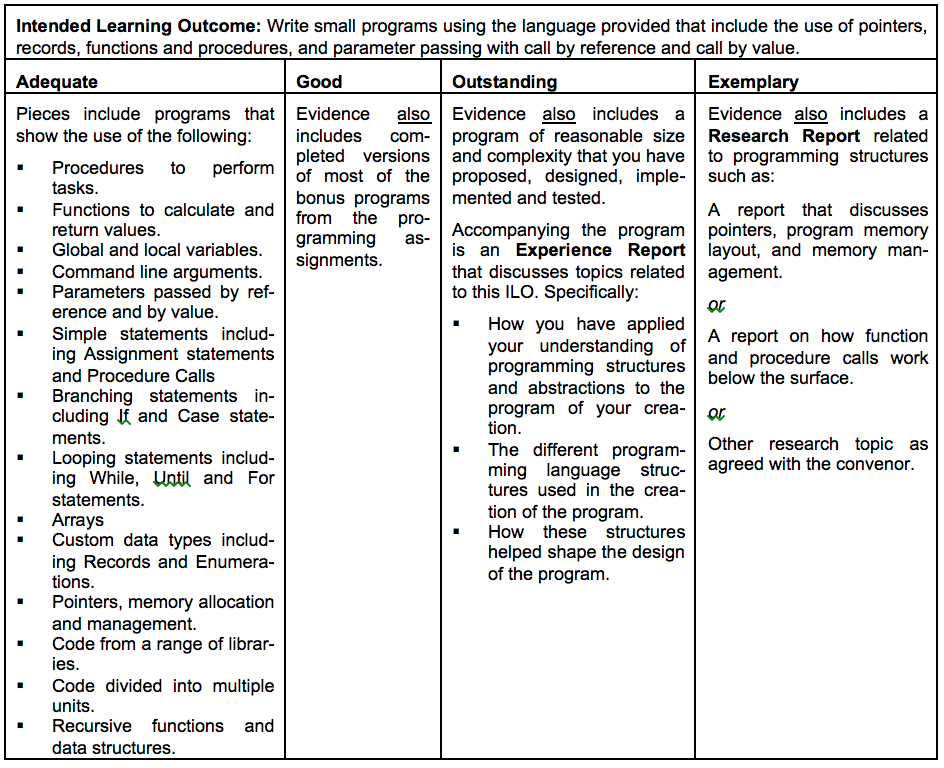
\includegraphics[width=0.95\textwidth]{AssessmentCriteriaDetail}
	\caption{Example assessment criteria related to a single intended learning outcome}
	\label{fig:i6_assessment_criteria_detail}
\end{figure}

At the same time, the resources used to support the teaching of these units were also developed. Resources for Introductory Programming (A) were developed during its delivery in Iterations 3, 5 and 6, as outlined in the following list.
\begin{enumerate}[noitemsep,nolistsep]
  \item Iteration 3:
  \begin{itemize}[noitemsep,nolistsep]
    \item A first version of the ``Programming Arcana'' book was developed. This combined the syntax diagrams from the Pascal Language Reference manual \cite{FPC:2013lang} with the notes that had previously been embedded within the lecture slide handouts.
    \item Students continued to be introduced to SwinGame later in the semester, with a number of students choosing to develop custom SwinGame projects for higher grade outcomes. 
  \end{itemize}
  \item Iteration 5:
  \begin{itemize}[noitemsep,nolistsep]
    \item Optional tasks were added to week 1 that encouraged students to start using SwinGame, and to go beyond the ``basics''.
    \item The Learn Programming with SwinGame video podcasts were created and delivered to students during the delivery of the unit.
    \item A template was provided for the Reflective Report (which later became the Learning Summary Report), see \fref{fig:i5_template}. The template provided a coverage matrix for students to indicate how well they believed their portfolios had met each of the intended learning outcomes. This was followed by sections for each intended learning outcome where students documented how the specific pieces they had included demonstrated they had achieve the outcome to the level indicated in their coverage matrix.
  \end{itemize}
  \item Iteration 6:
  \begin{itemize}[noitemsep,nolistsep]
    \item Templates were provided for each of the short reports that were required to meet the Good standard for each intended learning outcome.
    \item The Learning Summary Report template was expanded to include a specific section for students to reflect upon their learning.
  \end{itemize}
\end{enumerate}

\begin{figure}[p]
  \centering
  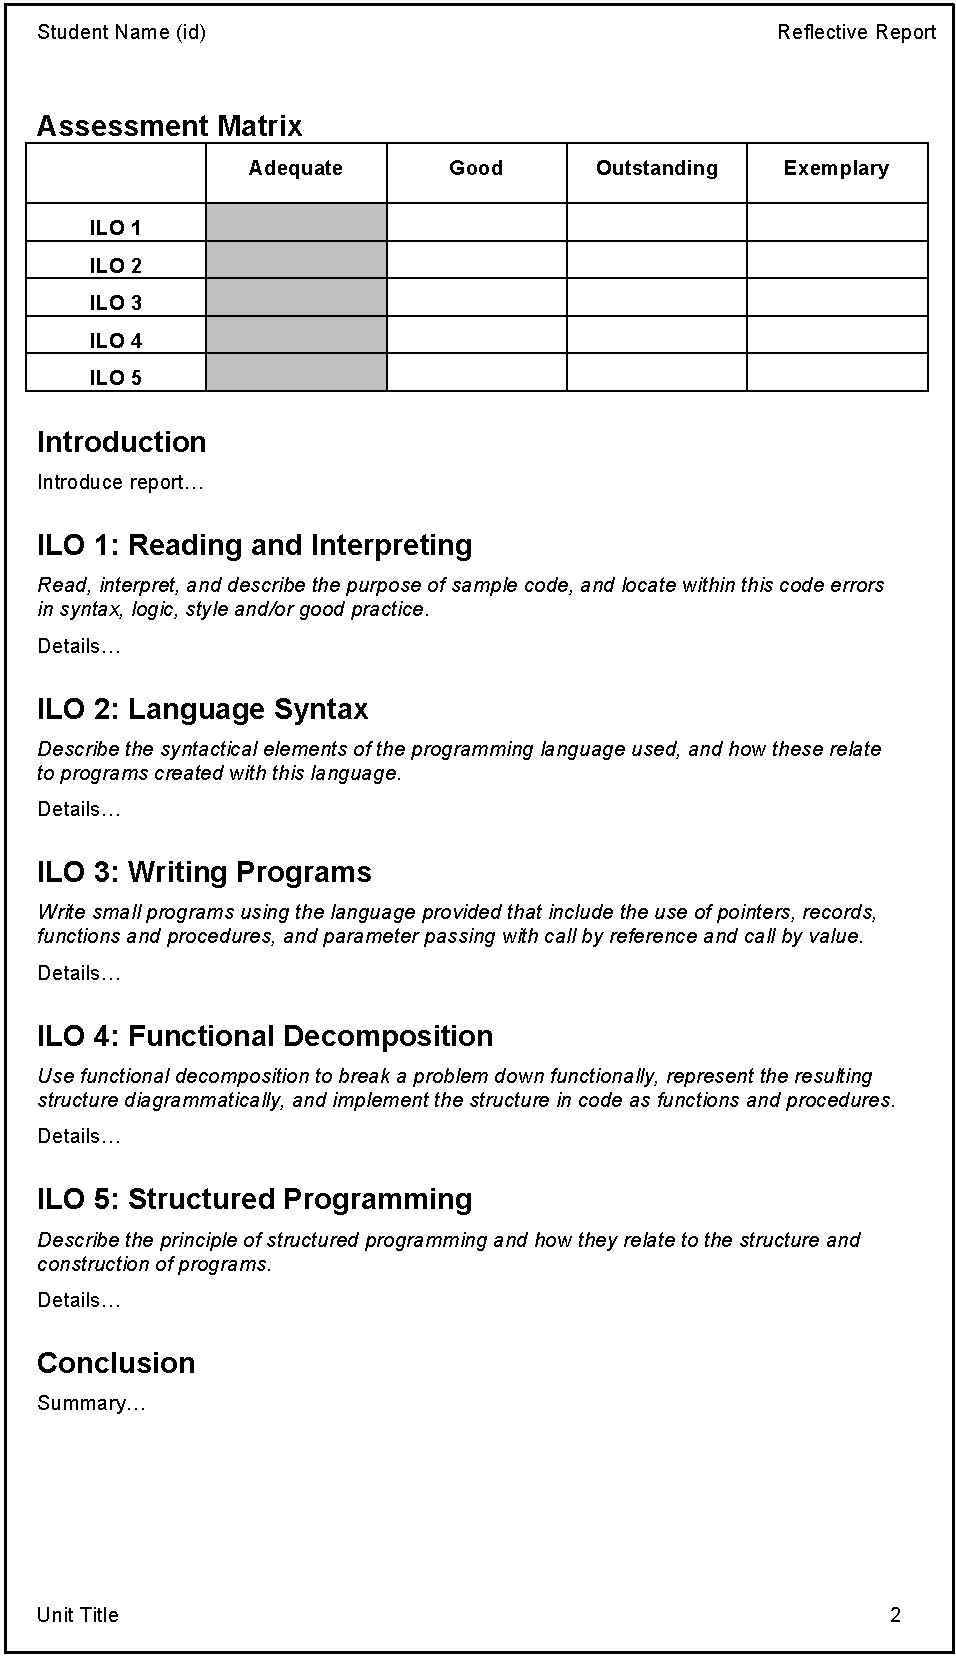
\includegraphics[width=0.8\textwidth]{I5Template}
  \caption{Main contents page from the template provided in Iteration 5}
  \label{fig:i5_template}
\end{figure}


Resources for Object Oriented Programming (A) were developed during its delivery in Iteration 4:
\begin{itemize}[noitemsep,nolistsep]
	\item Additional video podcasts were created to add support for the newly introduced Objective C programming language.
	\item Rather than develop a custom text, a range of textbooks and online resources were made available to students. This enabled the support of a range of languages, without the student overhead of developing additional resources.
	\item Previous exercises distributed to students with the lecture notes were moved online.
\end{itemize}

% subsubsection plan (end)

\paragraph{Data} % (fold)
\label{ssub:data_3_6}

\fref{fig:intro_prog_1_9} shows the grade distributions for Introductory Programming (A). The pass rate improved over these iterations: from 69\% in Iteration 1, to 72\%, 77\%, then 80\% in Iteration 6. At the same time the percentage of students receiving Distinction and High Distinction grades decreased from 57\% in Iteration 1, to 42\% then 37\% and 23\% by Iteration 6. These results relate to the changes for the various iterations, with additional guidance and experience helping a greater number of students achieve passing grades, while tightening of criteria for higher grades required students to demonstrate progressively deeper learning over these iterations.

\begin{figure}[htbp]
  \centering
  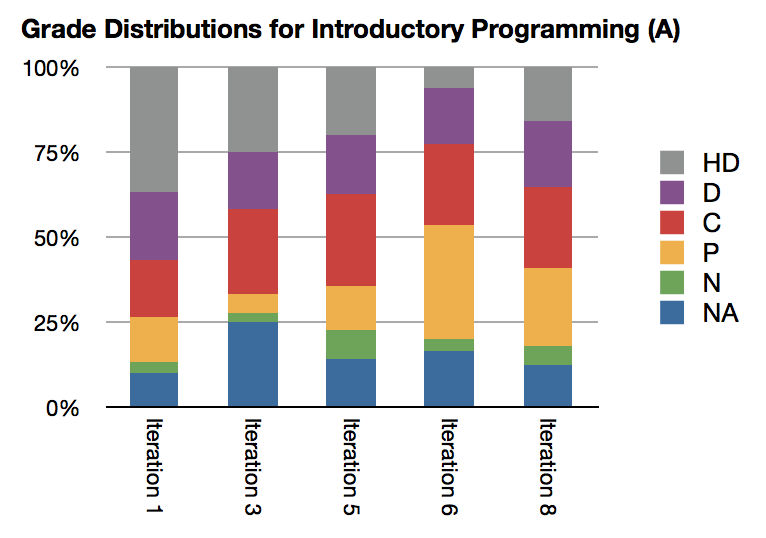
\includegraphics[width=0.8\columnwidth]{IntroProgA}
  \caption{Result distributions for Introductory Programming (A) from Iterations 1, 3, 5, 6 and 8.}
  \label{fig:intro_prog_1_9}
\end{figure}

\fref{fig:oop_1_9} shows the grade distributions for Object Oriented Programming (A). In Iteration 2 the pass rate was 69\%; this improved in Iteration 4 to 74\%. The percentage of students achieving Distinction and High Distinction dropped over this time from 29\% to 26\% in Iteration 4. As with the introductory programming unit, these results help demonstrate improvements in both guidance and expectations. 

\begin{figure}[htbp]
  \centering
  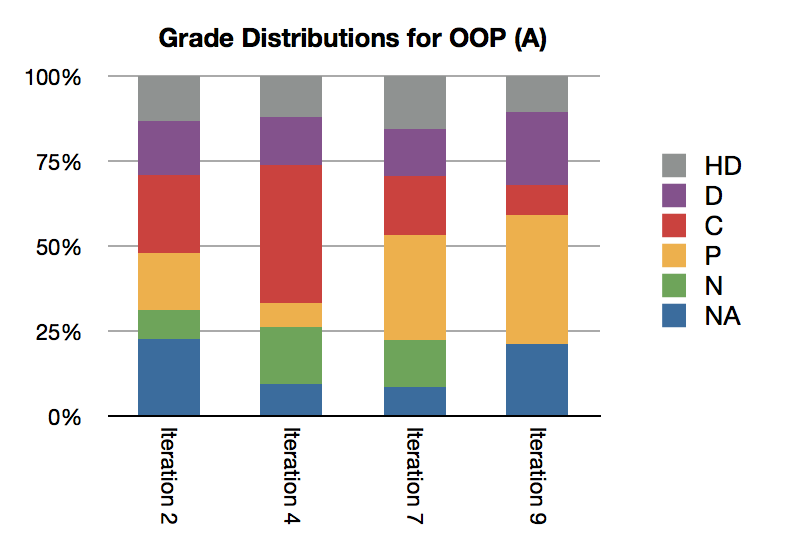
\includegraphics[width=0.8\columnwidth]{OOPA}
  \caption{Result distributions for Object Oriented Programming (A) from Iterations 2, 4, 7 and 9.}
  \label{fig:oop_1_9}
\end{figure}

% \begin{figure}[htbp]
%   \centering
%   \includegraphics[width=\columnwidth]{Iterations3to5}
%   \caption{Result distributions from Iterations 3 to 5.}
%   \label{fig:iterations_3_6}
% \end{figure}

% subsubsection data (end)

\paragraph{Reflections and Analysis} % (fold)

Staff reflections from these teaching periods indicated the improvements to assessment criteria had helped reduce the time needed to perform the portfolio assessment, and this improved with each iteration. In terms of student learning, the lost productivity from Iteration 2 was not present in these iterations and student portfolios demonstrated continually improving outcomes. We believe this can be attributed to our developing experience with portfolio assessment, student social sharing of their experiences, the improvements in the clarity of the assessment criteria, and the availability of prior portfolios as examples of what was required.

With these iterations we finally felt we were starting to receive the benefits we had hoped this teaching environment may achieve. Staff felt that student outcomes better matched their expectations, and that the quality of student work improved each semester as better guidance was provided.

\paragraph{Development of Principles} % (fold)

The environment created in Iterations 3 to 6 had aimed to address the issues identified in Iteration 2, and then worked on improving the assessment criteria and available resources. At the end of these iterations it was felt that portfolio use was an effective means of assessing student outcomes.

By the end of Iteration 6, it was apparent that the separation of assessment criteria by individual intended learning outcome was overly confusing, and had not productive for either staff or students aiming for higher grades. The criteria to meet the \emph{Outstanding} standard had required students to create a program of their own design. To achieve this, students had to apply their understanding of the concepts covered by the unit, but the assessment criteria had then required separate documentation for each intended learning outcome. This was time consuming for the students to prepare and for staff to assess. At the same time the separation of these reports made it difficult for students to relate to ``real world'' use of these concepts.

This experience influenced a number of the principles stated in \cref{cha:guiding_principles}. 

\begin{itemize}[noitemsep,nolistsep]
	\item The model had demonstrated an effective combination of constructive learning theories (\Pref{itm:construct}) and aligned curriculum (\Pref{itm:align}).
	\item Clearly communicating high expectations (\Pref{itm:expectations}) had helped with the Theory Y environment (\Pref{itm:theory_y}) and the focus on formative feedback (\Pref{itm:formative}).
	\item The use of a reflective component in the portfolios, which relates to \pref{itm:reflect}, had been positive, and helped students to reflect upon what they had learnt.
	\item Improvements in both how we taught and what we taught was greatly aided by reflective practice (\Pref{itm:reflect}) and the focus on creating a productive learning environment (\Pref{itm:agile}).
	\item The separation of the assessment criteria by intended learning outcome had negatively impacted on students ability to demonstrate depth of knowledge, working against \pref{itm:focus}.
\end{itemize}

% paragraph development_of_principles (end)


% subsubsection iterations_3_to_6 (end)

% subsection as_the_model_stabilised (end)
\clearpage
\subsection{Latest Iterations} % (fold)
\label{sub:latest_iterations}

Iterations 3 to 6 had started to demonstrate the benefits of portfolio-based assessment. Over these iterations the units had been delivered to students enrolled in a degree with a focus on computer science. At the start of Iteration 7 the university was looking to consolidate programming units, and it was decided to trial the portfolio assessment approach with engineering students, in Introductory Programming (B). As such, these iterations aimed to continue to develop the model while also testing it with a wider range of students.

\begin{enumerate}[noitemsep,nolistsep]
	\item Iteration 7: Introductory Programming (B) was taught using the C programming language.
	\item Iteration 8: The two introductory programming units were combined into a single unit. This used two programming languages, starting with Pascal and then moving to C later in the semester.
	\item Iteration 9: Combined together the two object oriented programming units. Prior to this iteration Object Oriented Programming (B) had been taught using a textbook style approach, focusing on language syntax, and was assessed using assignments and a final exam.
\end{enumerate}

\subsubsection{Iterations 7, 8, and 9} % (fold)
\label{sub:iterations_7_to_9}

\paragraph{Focus} % (fold)

The focus for iterations 7 to 9 was on expressing assessment criteria that required a consolidation of knowledge across the unit's intended learning outcome. In prior iterations, the separation of assessment criteria by individual intended learning outcomes, as illustrated in \fref{fig:i6_assessment_criteria_detail}, had been in conflict with the desire for students to demonstrate an integrated understanding of the concepts. The solution came in the realisation that higher grades could require students to apply the concepts related to the unit's intended learning outcomes in the development of a project of the students own design. The clarity of this helped in communicating expectations, and greatly simplified the assessment criteria. 

The second focus of these iterations was the incorporation of other units into this approach: Introductory Programming (B) and Object Oriented Programming (B). This increased the number of students to which this approach was delivered, and broadened the cohort to include students not necessarily interested in software development. This required a secondary focus on addressing issues of scale, and potentially additional issues related to plagiarism.

In relation to the principles stated in \cref{cha:guiding_principles}, \tref{tbl:prin_iter_7_9} illustrates the principles on focus for each iteration. Limitations identified in Iteration 6 resulted in changes to the expectation (\Pref{itm:expectations}) of students, and the focus (\Pref{itm:focus}) of the formative feedback process (\Pref{itm:formative}). At the same time, the larger class numbers renewed the need for productive learning environments (\Pref{itm:agile}), and the further use of multiple languages helped guide the clear focus on concepts (\Pref{itm:concepts}).

\begin{table}[h]
  \centering
  \caption{Principles related to Iterations 7 to 9: focus \foci, present \done, partially present \some.}
  \label{tbl:prin_iter_7_9}
  \begin{tabular}{l|ccccccccc|ccc}
    Iteration & \Pref{itm:construct} & \Pref{itm:align} & \Pref{itm:formative} & \Pref{itm:focus} & \Pref{itm:expectations} & \Pref{itm:support} & \Pref{itm:theory_y} & \Pref{itm:agile} & \Pref{itm:reflect} & \Pref{itm:paradigm} & \Pref{itm:concepts} & \Pref{itm:authentic} \\
    \hline
    %               P1      P2      P3      P4      P5      P6      P7      P8      P9     P10     P11     P12
    Iteration 7 & \done & \done & \foci & \foci & \foci & \done & \done & \foci & \done & \done & \foci & \done \\
    Iteration 8 & \done & \done & \done & \done & \done & \done & \done & \done & \done & \done & \done & \done \\
    Iteration 9 & \done & \done & \done & \done & \done & \done & \done & \done & \done & \done & \done & \done \\
  \end{tabular}
\end{table}

\paragraph{Action Plan} % (fold)

For these iterations the assessment criteria was as reported in \cref{cha:example_impl} and shown in \fref{fig:assessment_criteria}. This was accompanied by an explanation of what was required from the individual components: weekly tasks, tests, own program, and research report. 

For the assessment criteria, the main challenge in iterations 7 to 9 had been on trying to find clear requirements for the Credit grade. This needed students to demonstrate good coverage of the intended learning outcomes, while limiting the required workload. The following list shows what was used as the criteria for the Credit grade over these iterations.

\begin{itemize}[noitemsep,nolistsep]
  \item Iteration 7: Students were required to complete a piece of their own creation that demonstrated good coverage of all intended learning outcomes. The Unit Outline was not specific, but suggested that this could include reports, concept maps, glossaries, or any other piece the student wanted to create.
  \item Iteration 8 and 9: Weekly tasks included core tasks, and extension tasks. The core tasks included strong guidance, whereas the extension tasks required a greater level of independence. The Credit grade required all weekly tasks to be completed, as well as a selection of the weekly extension tasks. This also kept the other piece of the students own creation as in Iteration 7. \fref{fig:i9_assessment_criteria} shows an example of the assessment criteria from Introductory Programming (B) in Iteration 9.
\end{itemize}

In terms of teaching and learning resources, these iterations included the redevelopment of a number of resources, and the development of the Doubtfire task tracking system.

\begin{enumerate}[noitemsep,nolistsep]
  \item Iteration 7: 
  \begin{itemize}[noitemsep,nolistsep]
  	\item A new version of the Programming Arcana was created. This version used SwinGame and focused on procedures first and the C programming language.
  	\item SwinGame was used from week 1 in core lab tasks, enabling the procedures first approach.
  	\item Syntax diagrams created for the Programming Arcana were used in the Lecture slides.
  	\item Weekly exercises were moved into the Programming Arcana to help encourage student to make greater use of the resource.
  	\item The Introductory Programming video podcasts were created to support the lecture material.
  \end{itemize}

  \item Iteration 8:
  \begin{itemize}[noitemsep,nolistsep]
  	\item The new Programming Arcana was extended to include both the C and Pascal programming languages.
  	\item Weekly exercises were moved back into the laboratory handout for a number of reasons including practicalities related to changes, and issues with student engagement. Changing the exercises in the Programming Arcana required the entire text to be recompiled and re-distributed to students, which made it more difficult to make changes during the delivery of the unit. Students also seemed less engaged with these exercises, and appeared to view these as ``textbook questions'' that could be skimmed over -- as they were related to the ``textbook'' not specifically designed for the unit. 
  	\item Additional documentation was provided to demonstrate the research process, and how a small research project could be conducted and documented.
  \end{itemize}

  \item Iteration 9:
  \begin{itemize}[noitemsep,nolistsep]
  	\item Weekly exercises were adjusted to include Lab exercises, Core exercises, and Extension exercises. The Lab exercises were designed to be worked through in a laboratory class with the guidance of a tutor. These exercises did not need to be included in student portfolios.
  	\item The Doubtfire tool was developed, and Core exercises were used as the weekly tasks for the burn down charts. To be eligible for Credit students needed to have all Core exercises signed off.
  \end{itemize}
\end{enumerate}


% subsubsection plan (end)

\paragraph{Data} % (fold)

For software development students the pass rate continued to rise through these iterations, with 82\% of students passing Introductory Programming (A) and 79\% passing Object Oriented Programming (A) in Iteration 9.

In Iteration 7, Introductory Programming (B) was introduced and achieved a 71\% pass rate. However, student portfolios were generally considered to be weaker than for those in Introductory Programming (A) and fewer students achieved high grades. This can also be seen in \fref{fig:combined}, which shows the results for the combined units in iterations 8 and 9.

\begin{figure}[htbp]
  \centering
  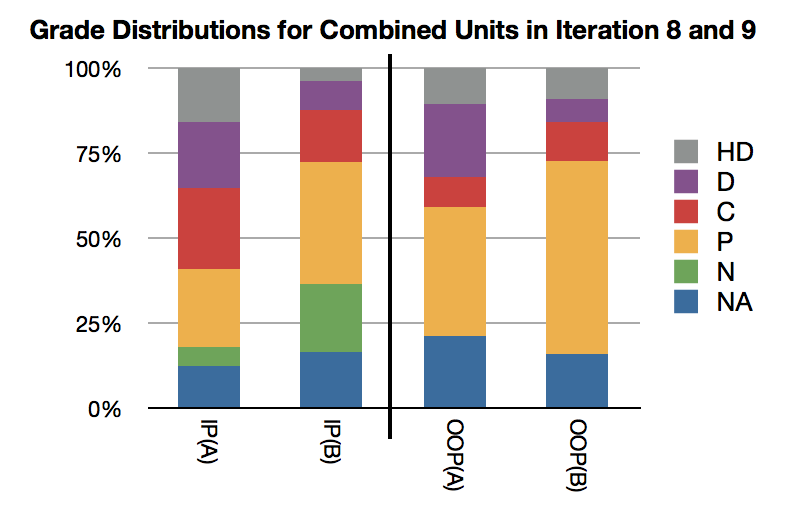
\includegraphics[width=0.8\textwidth]{CombinedUnits}
  \caption{Result distributions for combined units in iterations 8 and 9}
  \label{fig:combined}
\end{figure}

\paragraph{Reflections and Analysis} % (fold)

With Introductory Programming (A) the quality of submitted portfolios continued to improve through these iterations. In Iteration 8 extra guidance was provided on how to conduct and document a small research project, and this seems to have been beneficial with an increased number of High Distinction portfolios.

With other student cohorts, the results seem less positive. Staff indicated a difficulty in engaging students not enrolled in a degree that focused on software development. This was most pronounced in the combined introductory programming unit, as can be seen in \fref{fig:combined}. Given that both groups of students had been delivered the same material, in the same classes, it had been assumed that the distribution of results should be similar. 

% A one-way analysis of variance (ANOVA) was used to test for differences in results amongst the different student cohorts. Results from the units differed significantly across the two cohorts, F (1, 219) = 28.94, p = 0.0000. These results are discussed further in \sref{sec:evaluating_progress_using_burndown_charts}.

% \begin{figure}[htbp]
%   \centering
%   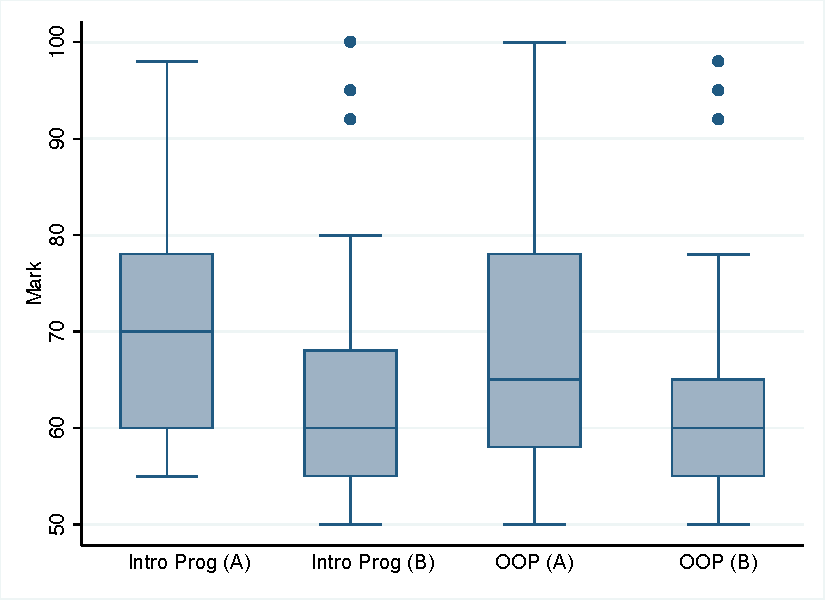
\includegraphics[width=0.8\textwidth]{CombinedUnitsBox}
%   \caption{A box plot showing the distribution of results across the two combined units}
%   \label{fig:combined_box}
% \end{figure}

The clarity of the assessment criteria and the clear delineation of what is required for the Pass, Distinction and High Distinction grades further reduced the time needed for staff to assess the portfolios.

While staff felt that the portfolio assessment was very successful through these iterations, the criteria for the Credit grade remained unclear and tended to require students to complete \emph{more work} rather than demonstrate \emph{better understanding}.

\paragraph{Development of Principles} % (fold)

These iterations followed the model described in \cref{cha:approach}, and delivered the units as outlined in \cref{cha:example_impl}. Implementations across these iterations embodied all of the principles from \cref{cha:guiding_principles}. The focus on creating a productive learning environment incorporating reflective practice (\Pref{itm:agile} and \Pref{itm:reflect}) continued to ensure that the process itself improved in each iteration.

% \begin{table}[h]
%   \centering
%   \caption{Principles related to Iterations 1 to 9. Focus is indicated by \foci, \done indicates in form presented in \cref{cha:guiding_principles}, \some indicates partially present but neither in planned focus nor in final form.}
%   \label{tbl:prin_per_iter}
%   \begin{tabular}{l|ccccccccc|ccc}
%     Iteration & \Pref{itm:construct} & \Pref{itm:align} & \Pref{itm:formative} & \Pref{itm:focus} & \Pref{itm:expectations} & \Pref{itm:support} & \Pref{itm:theory_y} & \Pref{itm:agile} & \Pref{itm:reflect} & \Pref{itm:paradigm} & \Pref{itm:concepts} & \Pref{itm:authentic} \\
%     \hline
%     %               P1      P2      P3      P4      P5      P6      P7      P8      P9     P10     P11     P12
%     Iteration 1 & \foci & \foci & \none & \some & \none & \done & \none & \some & \none & \done & \some & \done \\

%     Iteration 2 & \foci & \foci & \foci & \some & \none & \done & \foci & \foci & \none & \done & \some & \done \\

%     Iteration 3 & \foci & \foci & \foci & \foci & \foci & \done & \foci & \foci & \foci & \done & \some & \done \\
%     Iteration 4 & \done & \done & \some & \some & \some & \done & \some & \some & \some & \done & \some & \done \\
%     Iteration 5 & \done & \done & \some & \some & \some & \done & \foci & \some & \foci & \done & \some & \done \\
%     Iteration 6 & \done & \done & \some & \some & \some & \done & \done & \some & \done & \done & \some & \done \\
 

%     Iteration 7 & \done & \done & \foci & \foci & \foci & \done & \done & \foci & \done & \done & \foci & \done \\
%     Iteration 8 & \done & \done & \done & \done & \done & \done & \done & \done & \done & \done & \foci & \done \\
%     Iteration 9 & \done & \done & \done & \done & \done & \done & \done & \done & \done & \done & \done & \done \\
%   \end{tabular}
% \end{table}

% subsection iterations_7_to_9 (end)

% subsection latest_iterations (end)

\subsection{Current Iteration} % (fold)

\paragraph{Focus}
This teaching approach is currently being used to deliver Iteration 10. In this iteration the focus is on achieving better outcomes in the combined units, and to reduce the workload required by the Credit criteria while still maintaining the a high standard.

As with iterations 7 to 9, Iteration 10 incorporates all of the principles outlined in \cref{cha:guiding_principles}. Similarly, Iteration 10 is using the model described in \cref{cha:approach}, and incorporates all activities and guidelines. The exemplar units from \cref{cha:example_impl} are based the units being delivered in this iteration.

Iteration 10 differs from Iteration 9 only in its strengthening of the use of the Glossary as the criteria for Credit.

\paragraph{Plan}
One of the success stories from Iteration 9 was the use of a Glossary covering programming terminology, abstractions, and statements. This was used as a means of getting students to \emph{describe} and \emph{explain} principles and associated concepts, and seemed to be an effective means of both engaging the students with the material and assessing their learning outcomes. As a result, Iteration 10 will use the glossary for the Credit criteria. It is hoped this will help students engage appropriately with the teaching and learning activities.

% subsection  (end)

\subsection{Summary} % (fold)
\label{sub:action_summary}

This section has presented results and analysis from nine iterations of an action research project that examined the implementation of portfolio assessment. The overall focus of this work was on development, application, and ongoing evaluation of the model from \cref{cha:approach}.

Initial attempts at portfolio assessment failed to demonstrate expected outcomes, and student portfolios were generally weaker than desired. Over subsequent iterations, assessment criteria were evolved to more tightly define what was expected of each grade and students portfolios improved to meet these expectations. In the later iterations, staff were able to quickly assess portfolios, and felt that grades accurately reflected student outcomes.

This work provides additional evidence of the strength of portfolio assessments for assessing and supporting learning. In each iteration the assessment criteria helped guide students in preparing their portfolios, and as the criteria evolved the evidence in student portfolios improved. Experience delivering portfolio assessed units resulted in criteria that clearly relates to active verbs at the multi-structural and relational levels of the SOLO taxonomy, providing a strongly aligned assessment of intended learning outcomes.

Our experience highlights the importance of ensuring intended learning outcomes are expressed clearly, and capture the core concepts and principles that need to be demonstrated in student portfolios. The assessment criteria then maps the intended learning outcomes to statements of required levels of achievement. Together the intended learning outcomes and assessment criteria express what needs to be done and how well it needs to be done by the students to achieve different grades.

The model presented in \cref{cha:approach} provided an effective means of achieving constructive alignment. For students the process provides support and encouragement through iterative formative feedback, gives them clear expectations of what they need to achieve, and results in meaningful grades. After the initial investment, the intended learning outcomes and assessment criteria provided a dual means for staff to express expectations, and the resulting environment encouraged reflective practice. During the teaching period, staff and student efforts were both directed toward the one goal: helping students achieve the intended learning outcomes to the best of their ability.

% subsection discussion (end)

% section lessions_learnt_from_action_research (end)
\clearpage
\section{Issues Identified in Student Reflections} % (fold)
\label{sec:issues_identified_in_student_reflections}

Student reflections provide a rich opportunity to identify issues that are relevant from the students' perspective. The investigation presented in this section analyses issues identified in student reflections from the Introductory Programming (A) unit in Iteration 6, and provides support for recommendations to help inform the development of units using this approach. 


\subsection{Method} % (fold)
\label{sub:issues_method}

This study examined student reflections from the Introductory Programming (A) unit from Iteration 6, the current iteration at the time of the study. It was decided to use portfolios from a single iteration for a number of reasons. Time was a primary consideration, with the thematic analysis being a time consuming process. By limiting the analysis to a single iteration this would also provide a snapshot of issues related to this particular iteration. Future studies could then repeat the analysis for future iterations, with this first study providing a point of comparison.

This section is divided into three parts to clearly describe the details of \emph{Introductory Programming (A) in Iteration 6}, the \emph{Student Cohort and Research Participation}, and the \emph{Thematic Analysis of Reflections}. In the Introductory Programming Unit section we provide details of the unit that was investigated as part of this research. The Student Cohort and Research Participation section details the student body undertaking this unit and how they were recruited to be part of this research. Finally the Thematic Analysis of Reflections section outlines the process followed to extract and analyse the data from the student portfolios.

\subsubsection{Iteration 6: Introductory Programming (A)} % (fold)
\label{sub:intro_prog_i6}

In Iteration 6, Introductory Programming (A) had implemented the large majority of the principles and processed discussed in \cref{cha:guiding_principles} and \cref{cha:approach}. The teaching and learning activities differed slightly from the introductory programming unit described in \cref{cha:example_impl}, though the emphasis on concepts over syntax was present. The topics for the twelve lectures for this teaching period are shown in the following list as they relate to the topics mentioned in student reflections.
\begin{enumerate}[noitemsep,nolistsep]
  \item Programs, Procedure, Compiling and Syntax
  \item User Input and Working with Data
  \item Functions, Procedures, and Parameters
  \item Branches and Loops
  \item Custom Data Types
  \item Functional Decomposition
  \item Case Study
  \item Pointers and Dynamic Memory Management
  \item Structured Programming
  \item Recursion and Backtracking
  \item Portfolio Preparation
  \item Review and Future Studies
\end{enumerate}

The unit's delivery included an early introduction topic of ``understanding syntax'', where students were taught how to read programming language syntax using the visual ``railroad'' diagram syntax notation. This allowed later lecture topics to focus on concepts, with syntax being offloaded to programming demonstrations and supplied notes, which included railroad diagrams and small code examples for each programming statement.

As described in \cref{cha:example_impl}, the allocated classes were designed with the goal of actively engaging students. Lectures typically included a review of previous topics, a short presentation using ``Beyond Bullet Points'' style lecture slides, an interactive programming demonstration, and group activities. Laboratory sessions involved code reading activities, guided coding activities, and practical hands-on exercises.

The approach to assessment included weekly submissions and formative feedback to help students develop their understanding, three hurdle tests to ensure basic competence, and portfolio assessment for final grades.

Students were asked to reflect on their learning in a Learning Summary Report, and a template document was provided to assist students in preparing their comments. The template prompted students to describe the pieces they had included in their portfolio, to describe how these pieces related to the unit's intended learning outcomes, and then to reflect on what they had learnt from the unit.

To help students in writing their reflections, the following instructions were provided in the template. 
\begin{quote}
  \small
  Think about what you have learnt in this unit, and reflect on what you think were key learning points or incidents. Answer questions such as: What did you learn? What do you think was important? What did you find interesting? What have you learnt that will be valuable for you in the future? Which activities helped you most? Has this changed the way you think about software development? Did you learn what you wanted/expected to learn? Did you make effective use of your time? How could you improve your approach to learning in the future? Etc. 
\end{quote}

Note that there were no prompts for students to include details on issues they had encountered, meaning that any issues expressed should have been significant to the learning experience of the student.

\subsubsection{Student Cohort and Research Participation} % (fold)
\label{sub:issues_student_cohort}

In Iteration 6 the Introductory Programming (A) unit was undertaken by 84 students, 70 of whom submitted a portfolio for assessment. Participation in the research was voluntary, with informed consent being sought in lecture 11 as outlined in \sref{sub:addressing_ethical_concerns}.

\tref{tbl:issues_student_numbers} shows the number of portfolios made available to this research, the number that included comments related to the theme of ``issues'' and the distribution of grades. The grade distribution is also shown in \fref{fig:issues_grade_dist}, and will be discussed in \sref{sec:issues_discussion}.

\begin{table*}[p]
	\footnotesize
	\renewcommand{\arraystretch}{1.3}
	\caption{Portfolios submitted, issue comments and grade distribution.}
	\label{tbl:issues_student_numbers}
	\centering
	\begin{tabular}{l|c|c|c|c|c|c}
    % \hline
        ~                     & Total & HD & D & C & P & F  \\ \hline
        Submitted Portfolio   & 70    & 5                & 14          & 20     & 28   & 3     \\ % \hline
        Agreed to participate & 59    & 5                & 13          & 16     & 23   & 2     \\ % \hline
        Commented on Issues   & 35    & 2                & 6           & 11     & 14   & 2     \\ 
         - Learning Issues    & 26    & 2                & 3           & 9     & 12   & 1     \\ 
         - Programming Issues & 22    & 1                & 4           & 8     & 7   & 2     \\
		%\hline
	\end{tabular}
\end{table*}

\begin{figure}[thbp]
	\centering
	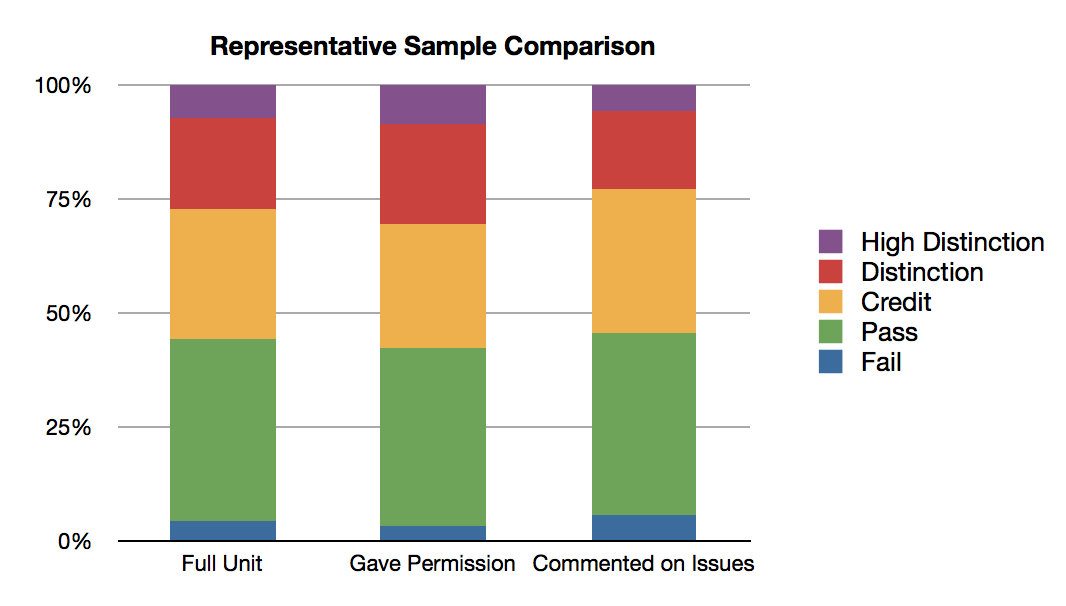
\includegraphics[width=0.8\textwidth]{IssuesGradeDistributions}
	\caption{Distribution of grades for the full unit, for those students who agreed to participate in the research, and for those who commented on issues.}
	\label{fig:issues_grade_dist}
\end{figure}



% subsection student_cohort (end)
% subsection introductory_programming (end)

\subsubsection{Thematic Analysis of Reflections} % (fold)
\label{sub:thematic_analysis_of_reflections}

The thematic analysis of student reflections followed the process outlined in \sref{sub:thematic_analysis}. Initial themes were generated by examining the reflective component of each portfolio and looking for all explicit mention of issues the student faced. Each new issue identified was matched to a theme and recorded in a spreadsheet. To ensure that all issues were reported in the results, the process of grouping themes did not remove or ignore any issues raised. All issues that could not be grouped into an existing theme were collected together as a miscellaneous ``other'' theme. The Results section outlines the different themes identified, and how these themes relate to the comments raised by students in their reflections.

% subsection thematic_analysis_of_reflections (end)
% section method (end)

\subsection{Results} % (fold)
\label{sec:issues_results}

A number of themes emerged from the analysis, and can be broadly classified as either general \emph{learning issues} or \emph{programming related issues}. (See \tref{tbl:issues_student_numbers} and \fref{fig:student_numbers}.) Each of these categories is presented in \tref{tbl:theme_counts} along with the number of students who raised these issues, broken down by grade. The following sections describe the individual themes in more detail.

\begin{table}[htbp]
	  \footnotesize
	  \renewcommand{\arraystretch}{1.3}
	
	\caption{Issue count results for grade and theme. Values of interest are indicated using bold format.}
	\label{tbl:theme_counts}
	\centering
	
    \begin{tabular}{l|p{5cm}|c|c|c|c|c|c}
    % \hline
        Theme                  & Description & Total & HD & D & C  & P  & F \\ \hline \hline
        Learning Issues        & Issues related to learning in general. &&&&& \\ %\hline
        - Time Issues            & Time constraints, or issues with time management.           & 14    & 1  & 0 & \textbf{5}  & \textbf{8}  & 0 \\ %\hline
        - Getting Started        & Comments relating to initial weeks, or tacking early hurdles.            & 8     & 0  & 1 & 2  & \textbf{5}  & 0 \\ %\hline
        - Learn through mistakes & Specifically commented on having issues and learning from these.           & 7     & 1  & 2 & 2  & 2  & 0 \\ %\hline
        - Other                  & Other learning related concepts not allocated to other themes.           & 5     & 0  & 0 & 2  & 2  & 1 \\ \hline
        Totals        & ~           & ~    & 2  & 3 & 11 & 17 & 1 \\ \hline \hline
        Programming Issues     & Issues related to programming topics, or technical areas.           & ~    & ~  & ~ & ~ & ~ & ~ \\ %\hline
        - Pointers               & Use of pointers and dynamic memory allocation functions.            & 11    & 1  & 2 & \textbf{4}  & 3  & 1 \\ %\hline
        - Parameters             & Mentions parameters, or parameter passing           & 8     & 0  & 1 & \textbf{4}  & 3  & 0 \\ %\hline
        - Program Design         & Algorithm and program structure design           & 7     & 0  & 1 & 1  & 3  & 2 \\ %\hline
        - Other (Syntax)           & Other issues, but related to the language syntax or concepts.           & 7    & 0  & 0 & 2  & 3  & 2 \\ %\hline
        - Other (General)                  & Other programming issues not allocated to other themes.           & 5    & 0  & 0 & 2  & 2  & 1 \\ %\hline
        - Recursion              & Declaration and use of recursive functions or data structures.           & 4    & 0  & 1 & 2  & 1  & 0 \\ \hline
        Totals     & ~           & ~    & 1  & 4 & 14 & 11 & 3 \\ % \hline
        
    % \hline
	\end{tabular}	
\end{table}

\begin{figure}[thbp]
	\centering
	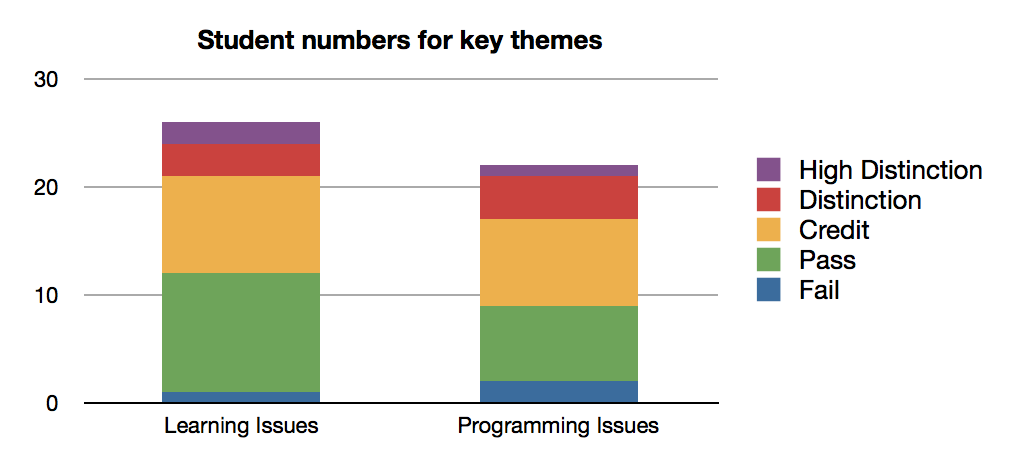
\includegraphics[width=0.8\textwidth]{NumStudentsMentioningIssues}
	\caption{Number of students mentioning learning issues and programming issues.  See \tref{tbl:issues_student_numbers}.}
	\label{fig:student_numbers}
\end{figure}

%TODO: SP noted that this is very info heavy. Still... i like it. :)

\subsubsection{General Learning Issues} % (fold)
\label{sub:general_learning_issues}

The \emph{general learning issues} capture all of the comments made by students that do not relate directly to a given programming topic or technical aspect of the unit, but instead relate to the students' learning experience in general. In this category the themes that appeared include  \emph{time management},  \emph{getting started} with the unit, and \emph{learning through mistakes}. The issue counts and grade distribution of these are included in \tref{tbl:theme_counts}, and can also be seen in \fref{fig:learning_issues}.

\emph{Time management issues} identified in the students' reflections included comments about aspects such as ``staying on task'', wishing they had ``asked for help earlier'', or the general need to improve their time management to enable them to achieve higher grades. It can be seen that the majority of these concerns were raised by students who obtained either a Pass or Credit grade. These comments are further supported by observations from teaching staff, who noted concerns about students not working consistently through the semester and not seeking help in a timely manner.

The next largest general learning issue was \emph{getting started} with programming. These comments specifically indicated issues related to the initial hurdle of getting started with the unit. One student noted this as their first experience using a computer, while others commented on the difficulty of the first few weeks' lab exercises. Again, these findings are supported by observations from the teaching staff who noted that a number of students withdraw from the unit before census date,\footnote{This is the date when the university records enrolment numbers, typically a few weeks after the start of the semester to allow for changes of enrolment.} and there was a general drop in enrolment numbers around this time. This may indicate that a larger number of students faced these issues but did not continue with the unit, though further work would be needed to verify this.

%% !!!! NOTE:  !!!! Not really an issue... how can we keep this in? I think it's important

The last main issue in this section related to students reflecting on the mistakes or struggles that provided them with an opportunity to learn something important, referred to as \emph{learning through mistakes}. For example, one student's reflection noted that:

\begin{quote}
``\ldots I suddenly gained insight [into the code] I had been struggling with \ldots''
\end{quote}

\noindent The reflection continued on to comment that having overcome these issues they gained a clearer understanding of the concepts taught up to that point, and that subsequent programs were easier to understand. 

The following \emph{other} issues were raised by individual students: 
\begin{itemize}[noitemsep,nolistsep]
	\item transitioning to university life and study,
	\item finding information in the online learning management system,
	\item seeking help in general,
	\item keeping up with the pace of the unit, noted as ``challenging but good'', and
	\item adjusting to portfolio assessment.
\end{itemize}
%TODO: added the "noted in one example" ... as the quote was unsupported. Hmm?

% subsection general_learning_issues (end)

\begin{figure}[htbp]
	\centering
	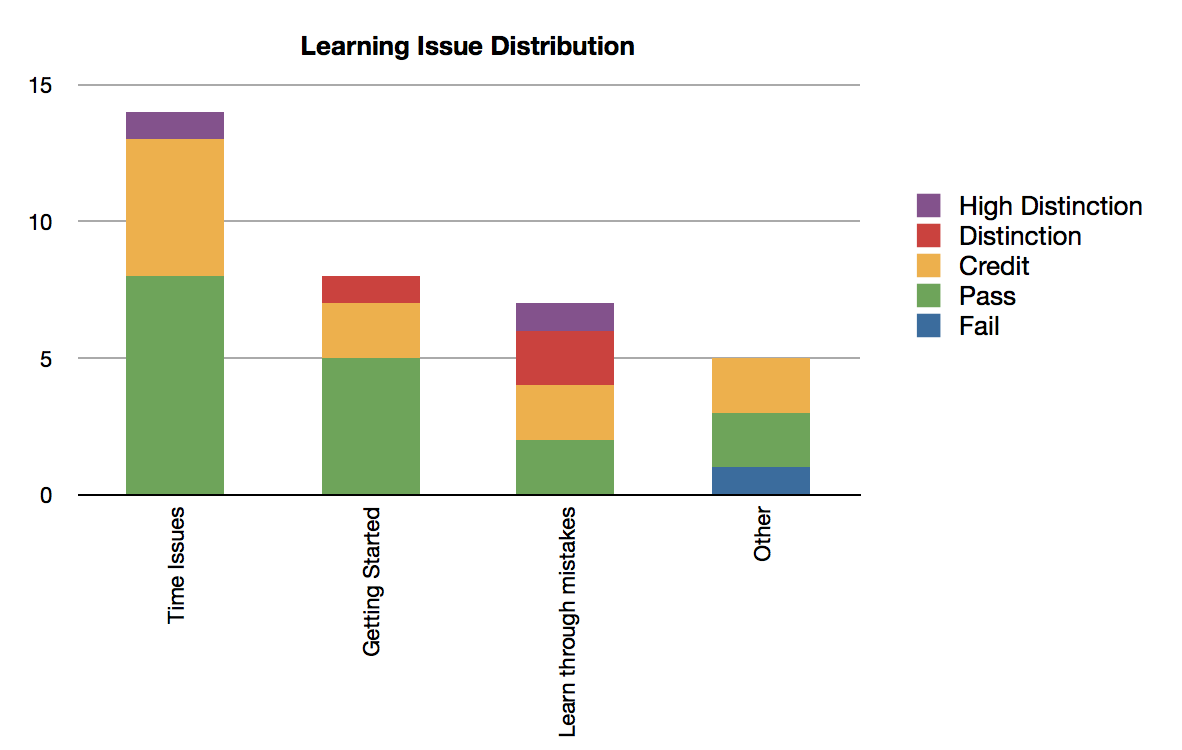
\includegraphics[width=0.9\textwidth]{LearningIssues}
	\caption{Number of students mentioning issues related to learning. See \tref{tbl:theme_counts}.}
	\label{fig:learning_issues}
\end{figure}


\subsubsection{Programming Issues} % (fold)
\label{sub:programming_issues}

As already mentioned, fewer students commented on programming or technical issues in their reflections than the more general learning issues. The programming sub-themes matched specific topics covered in the unit, including \emph{pointers}, \emph{parameters}, \emph{program design}, and \emph{recursion}. In this theme the \emph{other} sub-theme featured more prominently, with a larger range of issues being located in the reflections of only one or two students. The data for these themes is listed in \tref{tbl:theme_counts} and shown in \fref{fig:programming_issues}.

\begin{figure}[htbp]
	\centering
	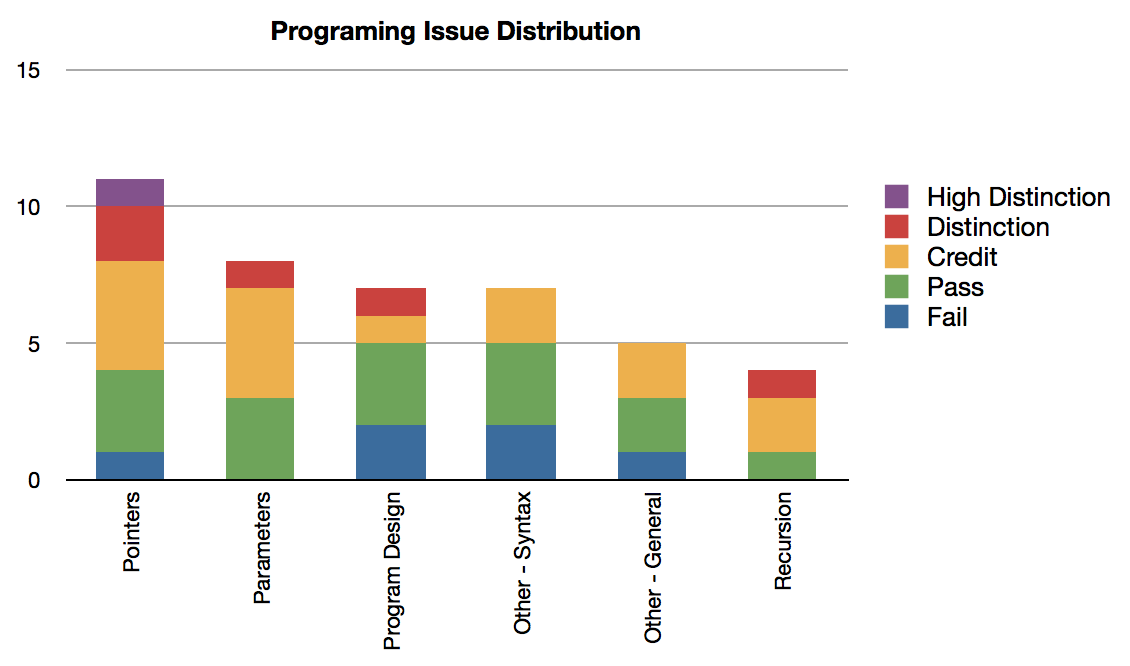
\includegraphics[width=0.9\textwidth]{ProgrammingIssues}
	\caption{Number of students mentioning issues related to programming. See \tref{tbl:theme_counts}.}
	\label{fig:programming_issues}
\end{figure}

Amongst the identified programming issues, \emph{pointers} featured most prominently. Comments typically referred to having issues with ``pointers'', with the more detailed comments discussing issues with knowing when to dereference pointers and being unsure of when to use pointers. This is further supported by notes from teaching staff indicating that pointers tended to be problematic even for students who demonstrated strong programming skills up to that point in the material.

\emph{Parameters} were also mentioned by a number of students as being a topic that was particularly challenging. This included comments relating to tracing parameter values through a number of function or procedure calls, and issues of a single value having different names across different routines. From these comments there is a direct connection from parameter issues to a student's understanding of program structure, or more importantly execution flow.

Issues relating to \emph{Program Design} were also raised in the portfolio reflections. These comments related to aspects such as using functional decomposition, planning program structure, and designing algorithms.

The \textbf{other} issues for the programming category captured issues identified by one or two students. These were classified as relating either to \textbf{syntax and concepts} or \textbf{general programming} issues.

\begin{itemize}[noitemsep,nolistsep]
  \item Syntax issues included:
  \begin{itemize}[noitemsep,nolistsep]
    \item iteration and working with loops,
    \item using arrays (two comments),
    \item creating composite data types using records,
    \item functions in general,
    \item dealing with syntax errors, and 
    \item using units to divide programs into multiple files.
  \end{itemize}
  \item General programming issues included:
  \begin{itemize}[noitemsep,nolistsep]
    \item ``programming in general'',
    \item ``following program code'' in code reading exercises,
    \item difficulties finding and using resources from the SwinGame library, and
    \item the maths needed to achieve programming tasks.
  \end{itemize}
\end{itemize}

There were also a number of reflections that raised the topic of \textbf{recursion}; these mentioned issues with both recursive functions and data structures. 

% subsection programming_issues (end)
% section results (end)

\subsection{Discussion} % (fold)
\label{sec:issues_discussion}

\subsubsection{Investigation Focus and Sample Quality}
% context
Comments provided by students, when reflecting on their learning during any unit, can be valuable and interesting in many ways, especially with respect to the evaluation of a particular approach to teaching. Our investigation focused specifically on the theme of issues mentioned or identified by students in their reflective reports. Results of the thematic analysis, presented in Section \ref{sec:issues_results}, identified clear key themes. Additionally, several individual comments were selected.

% The quality of the data - good 
The analysis considered a sample of reflective reports presented in a single semester unit. Of the 70 students in the class, almost 85\% were willing to participate. Within the participant group, 35 students wrote one or more comments that matched the target theme. \tref{tbl:issues_student_numbers} and \fref{fig:issues_grade_dist} show that the relative distribution of grades in the contributing group matches closely to both the participant group and the entire results for the unit. This strongly supports that the results are a representative sample of the unit, at least with respect to grade distribution. 

% Is is possible that the sample is not representative of students who like to keep to themselves and tend to communicate less.

\subsubsection{General Learning Versus Programming Issues} % (fold)
\label{sub:balance_of_learning_versus_programming_issues}

Beginning with the two key themes of general learning issues and programming issues (\tref{tbl:issues_student_numbers} and \fref{fig:student_numbers}) it can been seen that the distribution of student grades is very similar, with a slightly stronger representation of Pass students in the learning issues theme.

Overall, more students commented on learning in general. This is of particular interest given the relative emphasis of the course material, which focuses on teaching programming concepts over syntax details. Despite the relatively small time spent on syntax, students did not mention having related issues.

A closer examination of the issues related to programming strengthens this analysis further. Most student comments on programming issues (\tref{tbl:theme_counts}) concerned applying programming concepts, rather than issues of understanding syntax. Also, these comments were about when and how to use the related programming concepts rather than specifically how to apply the syntax of the language used. 

Comparison of the grade distributions within the learning issues (\fref{fig:learning_issues}) and programming issues (\fref{fig:programming_issues}) suggests potentially interesting differences, such as issues specific to grade groups, and other issues across all grades. The sample size of this investigation limits any significant insight although some points are listed in later discussion.

% subsection balance_of_learning_versus_programming_issues (end)

\subsubsection{Learning Issues}

\paragraph{Time Management} % (fold)
\label{ssub:time_management}

issues were identified by the largest number of students (\tref{tbl:theme_counts}). The grade distribution is skewed towards student's who achieved Pass and Credit results (bold values), suggesting that students who do achieve Distinction or High Distinction results managed time better, and that the unit structure requires good time management to achieve these outcomes.

Developing a portfolio that demonstrates the ability to apply concepts taught requires time: time to practice using the concepts, and time to demonstrate their use competently. For students to achieve Distinction and High Distinction grades, they needed to be able to organise their time effectively. 

With more traditional forms of assessment, marks can be used as incentives. Using assessment due dates during the delivery of the unit has the effect of turning marks into time distributed weighted incentives. Marks no longer represent the importance of the learning outcome, but match allocation of incentive. Consider, for example, the allocation of marks for lab attendance. These marks do not help measure the students' learning outcomes, but are purely there to incentivise lab attendance. Similarly, assignments due within the unit delivery period assess the speed of acquiring and demonstrating the required knowledge. 

With portfolio assessment the summative assessment is delayed until after unit delivery. This has the benefit of providing a more direct assessment of learning outcomes, but has a cost related to loss of incentives during delivery. While this is positive from a learning perspective, it can easily lead to students delaying their work on portfolio assessed units in order to address what they perceive as more time critical assignments in other units. Given the number of comments related to this issue, it appears to be easy for students to then lose sight of how they are falling behind in a unit with a relatively flexible portfolio assessment.

The prevalence of issue provided the incentive to implement the Doubtfire tool described in \sref{sec:doubtfire}. The use of this tool is discussed in \ref{sec:evaluating_progress_using_burndown_charts}.

% subsubsection time_management (end)

\paragraph{Getting Started} % (fold)
\label{ssub:getting_started}

is another issue facing many students (\tref{tbl:theme_counts} and \fref{fig:learning_issues}). In the first few weeks of the semester, students face practical and conceptual issues. Practical issues include installing compiler software and text editors, learning to use command line tools, and issues with general computer use. At the same time students need to build a viable conceptual model of computing \cite{Hoc:1990}, and relate this to the programs they are creating. 

Early on students may also face challenges transitioning to university study and university life in general. In the first few weeks students are also more likely to have issues with syntax, and dealing with syntax errors. Together these challenges can present a significant hurdle for students.

These issues could be addressed in a number of ways. Shifting toward a single, easy to install, IDE could remove some issues related to the use of the command line compiler. However, IDEs are typically designed for professional audiences and would add overhead related to use of a more complex programming environment. These environments also obscure the underlying tools which and does not assist students in building their conceptual model of computing. The teaching staff also considered that students undertaking this unit do need to learn how to use a command line, and this early introduction meant that later units could expect at least some student familiarity with command line tools.

% subsubsection getting_started (end)

\paragraph{Learning Through Mistakes} % (fold)
\label{ssub:learning_through_mistakes}
%  - - learning through mistakes (constructivism) across all grade levels (suggestive)

The students' active role in building their own conceptual model of a topic plays a significant role in constructive learning theories \cite{Glasersfeld:1989}. Effective teaching then becomes the ability to place students in situations where errors in their understanding can be challenged to help the students build viable conceptual models. 

With this in mind it is interesting to note, as shown in \tref{tbl:theme_counts}, the number of students who commented on gaining significant understanding through making mistakes. In line with constructive thinking, these students encountered situations in which their conceptual model was inappropriate, and in addressing the associated problems they were able to gain a better, more robust, conceptual model.

Comments about learning through mistakes were distributed across all grades, from Pass through to High Distinction (\fref{fig:learning_issues}). This suggests that mistake-based learning experiences are beneficial to a wide range of students, albeit with some students gaining a better understanding than others through the process. 

% subsubsection learning_through_mistakes (end)


\paragraph{Other Learning Issues} % (fold)
\label{ssub:other_learning_issues}

From the other issues students noted, many can be attributed to transitioning to university education. For example, learning to locate and use learning resources and to seek help, are all issues that students must come to deal with when shifting to university education.

It is interesting to note that one student did raise a complaint about portfolio assessment, indicating that it would be easier to sit an exam. While this is only a single student, it does highlight that the purpose of the ongoing assessment may not be realised by all. \citet{Tang:1999} indicated that students tend to apply narrower learning strategies for examinations, focusing on memorising material covered in lectures. In contrast, \citet{Tang:1999} also found that with portfolio assessment students adopted a wider perspective, making use of higher cognitive activities such as application, relation, and reflection. Students are likely to find these higher cognitive activities more challenging, and therefore those who wish to apply surface learning approaches are likely to prefer other assessment strategies.

% subsubsection other_learning_issues (end)

\subsubsection{Programming Issues}

\paragraph{Pointers and Recursion} % (fold)
\label{ssub:pointers_and_recursion}

Our results support those from \citet{Lahtinen:2005} in indicating that students find learning pointers challenging. Issues related to using pointers and memory management featured across a range of grade results (\tref{tbl:theme_counts} and \fref{fig:programming_issues}), indicating that this concept was challenging even for those students who managed to achieve good results in the unit. 

Pointers require a good conceptual understanding of computing, and the mental ability to debug logical errors. Issues with pointers can often result in abrupt program termination, which can be very confronting for beginner programmers. Locating the cause of these errors is an additional challenge, that requires a students to build a mental model of what is happening within the programs they have written.

Issues with recursion were raised by fewer students than other issues, which is in contrast to the study by \citet{Lahtinen:2005}. This may be explained by the short time students had with recursion in this study. A deep exploration of recursion was not required for students to pass the unit. It is likely, therefore, that many students did not have sufficient time to explore more involved applications of recursion.

In addition to being complex, pointers and recursion both occur relatively late in the curriculum. With pointers, students had little time to develop the skills necessary to handle associated issues, whereas with recursion the short time meant students had little opportunity to develop programs of sufficient complexity to encounter issues.  In either case, at the time of writing their reflections, issues with later lecture topics are perhaps more likely to be in focus.

% subsubsection pointers_and_recursion (end)

% From the comments ... identified the following themes.
%  - Technical
% Programming General - pointers and parameters (minor recursion, arrays)

\paragraph{Parameters} % (fold)
\label{ssub:parameters}

require students to understand local scoping of variables, procedure and function calls, and methods for sharing these values between functions and procedures. This appears to be another point at which students need to expand their internal mental model of computing \cite{Hoc:1990}. 

While parameter concepts can take time to understand, issues are likely to be constructive in nature. When the logic for a program is contained within a single procedure, students can develop a simplistic model of what is occurring when other functions or procedures are called. When students need to design their own functions and procedures that require parameters, they are presented with situations that challenge their simplistic model. This suggests that parameters provide a significant learning opportunity from a constructive perspective.

The two different parameter passing methods are taught in the unit, with pass by reference being used to create procedures to swap parameter values, as well as allowing procedures to modify data within structures and arrays. Call by reference provides an early introduction to references. 
% Make point on parameters (link to research), suggests turning point in learning (link to constructivism), occurs early (week 3), suggests enabling concept


% subsubsection parameters (end)


\paragraph{Program and Algorithm Design} % (fold)
\label{ssub:program_and_algorithm_design}

Program and algorithm design are progressively taught throughout the unit, with the main focus being in the middle of the unit's delivery in topics related to functional decomposition and structured programming. Comments by students indicated several issues on how to practically apply the concepts covered to create programs. 

We initially expected a larger representation of this issue, as design tasks require a deeper \emph{relational} understanding of the concepts being used. However, the core tasks students had to submit for a Pass grade were accompanied with detailed instructions to help ease these design issues. Extension tasks required for a Credit grade did require some design components, and less guidance was provided. Students attempting their own program, necessary for a Distinction grade, needed to perform design activities as these programs were of their own design and creation.

% subsubsection program_and_algorithm_design (end)

\paragraph{Other Programming Issues} % (fold)
\label{ssub:other_programming_issues}

raised by students can be classified as individual challenges. It seems that students are likely to learn at different paces, in different ways, and find different topics challenging. Again, general comments concerned the application of programming concepts, rather than with programming language syntax itself. Each of the raised issues indicated a point at which students had an an awareness of these and an opportunity to challenge and develop their conceptual understanding of programming and their model of computing. 

% subsubsection other_programming_issues (end)

\subsubsection{Recommendations}
 
Based on the thematic results and on the experiences of staff involved in the unit delivery, there are a number of implications and recommendations that can be made. These recommendations are listed below, and their explanations follow.

\begin{itemize}[noitemsep,nolistsep]
	\item Strongly avoid mixing formative with summative assessment
	\item Give students time to adjust to portfolio assessment
	\item Focus on student ``awareness''
	\item Use a quick formative feedback process
	\item Avoid the ``tutor debugging'' phenomena
	\item Use visual methods to convey progress
	\item Make students aware of issues they are likely to face
\end{itemize}

These recommendations have been incorporated into the model described in \cref{cha:approach}, and in the exemplar units discussed in \cref{cha:example_impl}. For example, the use of the sign off process for core tasks aimed to raise student awareness, and is linked to the Doubtfire tool's visual burn down charts.

\paragraph{Always formative, lastly summative}

Separating formative feedback processes from summative marking has a clear value, and this is reflected in student comments. Our observation is that using a punitive marking system creates an incentive for students to hide faults and limits in their understanding. However, students need to know what they need to learn and need to expose their misunderstandings in order to help staff guide them in developing appropriate mental models. Related to this is the time a student may spend asking about marking schemes or lost marks -- time better spent on learning.

% It takes time...
\paragraph{Students need time to adjust}

In comments to staff, students have said that it takes time to get used to a portfolio based unit even if they understand the principles. If we consider that students are somewhat conditioned to respond to summative marking and due dates as a way of allocating their attention, an interesting question emerges: how do we help students maintain an active engagement with the unit activities without marks? The Doubtfire tool was one attempt at answering this question, though this remains an ongoing challenge and research opportunity.
 
\paragraph{Focus on student awareness}
 
Primarily, student awareness is the basis for positive engagement and an aware student has the opportunity to make appropriate choices. To support this, staff need to communicate the structure, activities and expectations of a portfolio-based unit to students as effectively as possible. Unfortunately students may essentially have poor habits that can take time to adjust. It is possible to help students with issues such as time management and, hence, learning outcomes.

Although formative activities many not have due date or marks (grade penalties), staff should still express clear expectations of when work needs to be done. In some cases this leverages a students' habits to their advantage as they feel compelled to do the work. Ideally, students should give these formative tasks as high a priority as assignments with marks.

\paragraph{Use quick formative feedback}

Very quick feedback helps to create strong reinforcement to each student that the process \emph{really is} formative and personally valuable. In a students' experience summative marking is often a delayed process. If formative feedback takes a long time it is removed from the students' current learning and challenges, and so can be confused as summative marking. Students need to be engaged with the formative nature of these assessments, making use of the feedback to help develop their understanding.

\paragraph{Avoid tutor debugging}

A possible problem with quick formative feedback, and resubmission opportunities, is that students may submit poorly prepared ``drafts'' and use staff simply to ``fix things''. This issue has been described as ``tutor debugging'' by some of our staff, and should be actively discouraged. One approach to this is to set minimum submission standards for work submitted for feedback. 

\paragraph{Use visual methods to convey progress }

Visual charting of tasks and completed work, calendar events and strong reminders of work and time limitations help to engage students. It is also possible that a ``gamefication'' approach, by recognising personal or group achievements and rewarding with awards, ``badges'' an other game-related concepts, can create a fun and personal incentive for students. We also recognise that there are also risks with gamefication, such as trivialisation of the value of core learning activities or distorting the value of learning activities through association to a gamefication artefact.

\paragraph{Tell students what to expect}
Finally, helping students understand the issues they are likely to face should help them prepare sufficiently for the more challenging tasks. This is particularly relevant to the issues related to getting started. The challenges early on in the unit may put a number of students off, and these students are likely to lose motivation and engagement with the unit. Making them aware that these challenges are ``normal'', and to be expected, may assist them in getting over early hurdles.

% section discussion (end)

\subsection{Summary} % (fold)
\label{sub:issues_summary}

In this section we have presented a thematic analysis of reflective reports presented by students as part of their assessment in the Introductory Programming (A) unit from Iteration 6. The development and delivery of the unit followed the model from \cref{cha:approach}, being an implementation of the introductory programming unit described in \cref{cha:example_impl}. A good representation of students distributed across all result grades agreed to participate in the study. 

Thematic analysis was directed specifically at the theme of \emph{issues} identified by students. Overall results showed that more students raised learning issues than programming related issues. Significant learning themes included time management, getting started and mistake-based learning. The most common programming issues were related to pointers and parameters, with only a small number of issues related to syntax, and both these results were expected. Issues related to program design were raised less than expected. 

The discussion considered a number of interesting results, and put forward recommendations and future directions for research in this area. 

% subsection summary (end)

% section issues_identified_in_student_reflections (end)

\clearpage
\section{Evaluating Progress using Burn Down Charts} % (fold)
\label{sec:evaluating_progress_using_burndown_charts}

The work presented in this section examines the rate of student progress, as recorded using the Doubtfire task tracking tool and reported in student portfolio. By examining the various rates of progress and grades associated with these portfolios, we are able to gain some insights into the teaching and learning environment, and provide recommendations to help inform the development of units using this approach. 

% Structure of Paper

% The following sections first outline the method used in conducting this research, providing details on the teaching and learning context, student cohort, method used for the analysis, and a brief overview of the online task tracking system. This is followed by the results from the data collection phase, and then the Discussion presents our interpretation and analysis of the data.

% section evaluating_progress_using_burndown_charts (end)


\subsection{Method} % (fold)
\label{sec:progress_method}

As with \sref{sub:issues_method}, this section is divided into three parts with the aim of clearly describing the teaching and learning context, the student cohort, and the details for the thematic analysis.

\subsubsection{Teaching and Learning Context} % (fold)
\label{sub:progress_teaching_and_learning_context}

This work analysed the progress of students from Introductory Programming (B) in Iteration 9. In Iteration 9, the teaching period consisted of thirteen weeks, twelve of which were teaching weeks, and a single week semester break in week six. Topics for the twelve lectures are shown in the following list.

\begin{enumerate}[noitemsep,nolistsep]
  \item Programs, Procedure, Compiling and Syntax
  \item User Input and Working with Data
  \item Control Flow: Branches and Loops
  \item Procedural and Structured Programming
  \item Arrays
  \item Custom Data Types
  \item Pointers and Dynamic Memory Management
  \item Learning a New Language  (C)
  \item Portfolio Discussion
  \item Arrays and Structures in C, and Recursion
  \item Pointers in C, and Backtracking
  \item Review and Future Studies
\end{enumerate}

An overview of the assessment criteria for Introductory Programming (B) in Iteration 9 is shown in \fref{fig:i9_assessment_criteria}. To be eligible for a pass grade students include a range of work of the weekly assessment tasks, and indicated how the pieces included demonstrated coverage of all intended learning outcomes. For Credit, student needed to complete all weekly assignments and include pieces that demonstrated good coverage of all intended learning outcomes. Distinction and High Distinction grades required students to go beyond these weekly tasks. Distinction grades were awarded for being able to apply the concepts learnt in the development a program designed by the student. High Distinction required students to undertake a small research project, and write this up in a short research report.

\begin{figure}[htbp] 
  \centering
  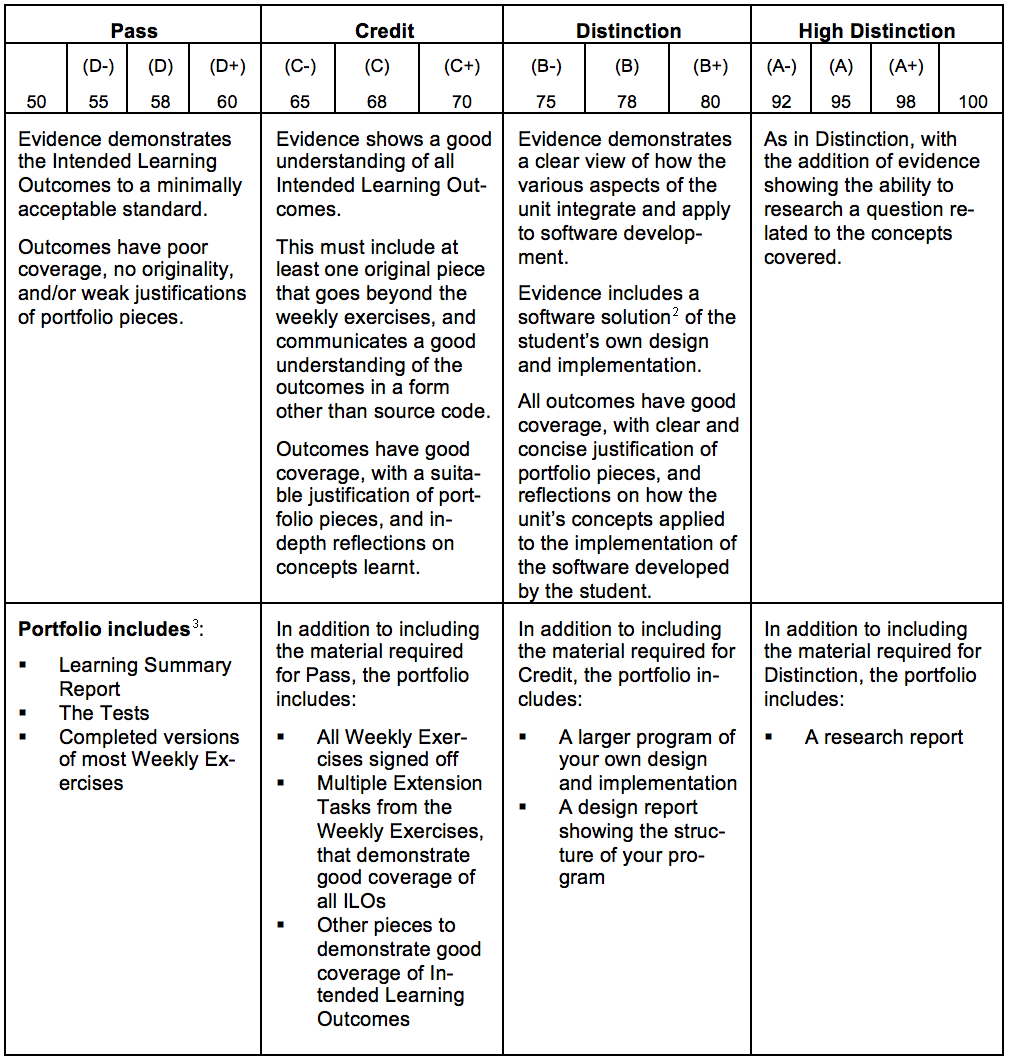
\includegraphics[width=0.8\textwidth]{AssessmentCriteria9}
  \caption{Overview of assessment criteria provided to students in the unit outline}
  \label{fig:i9_assessment_criteria}
\end{figure}

In Iteration 9, the Doubtfire tool was used to track student progress against the Core Tasks from the weekly exercises. An example of the charts from Introductory Programming (B) in Iteration 9 is shown in \fref{fig:progress_example_chart}. As described in \cref{cha:supporting}, the charts show the cumulative amount of work remaining week-by-week, which decreases as work is completed. 

\begin{figure}[thbp]
  \centering
  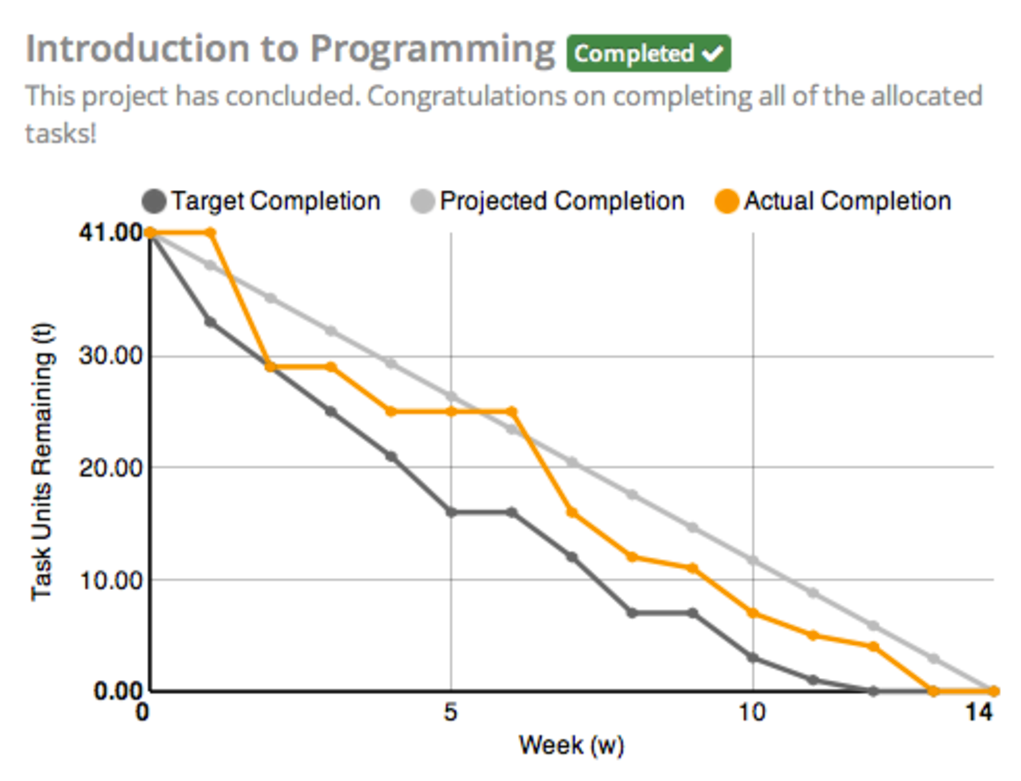
\includegraphics[width=0.8\textwidth]{ExampleChart}
  \caption{An example burn down chart from the online tool Doubtfire, showing progress against weekly tasks for Introductory Programming (B) in Iteration 9.}
  \label{fig:progress_example_chart} 
\end{figure}

% subsubsection use_of_doubtfire_in_the_unit (end)

\subsubsection{Student Cohort and Research Participation} % (fold)
\label{sub:progress_student_cohort}

At the end of the teaching period 139 students submitted portfolios for assessment. Of these, 87 agreed to participate in this research. Participation in the research was voluntary, with informed consent being sought using the process described in \sref{sub:addressing_ethical_concerns} in lecture 9.

\tref{tbl:progress_student_numbers} shows the grade distribution of the submitted portfolios, those made available to this research and of these, those who included their burn down chart in their portfolio.

\begin{table}[hbp]
  \footnotesize
  \renewcommand{\arraystretch}{1.3}
  \caption{Grade distribution of portfolios submitted}
  \label{tbl:progress_student_numbers}
  \centering
  \begin{tabular}{l|c|c|c|c|c|c}
    % \hline
        ~                     & Total & HD & D & C & P & N  \\ \hline
        Submitted Portfolio   & 139    & 7                & 25          & 24     & 79   & 4     \\ % \hline
        Agreed to Participate & 87    & 6                & 22          & 17     & 39   & 3     \\ % \hline
        Included Chart & 80 & 6 & 22 & 17 & 33 & 2 \\
    %\hline
  \end{tabular}
\end{table}

\begin{figure}[thbp]
  \centering
  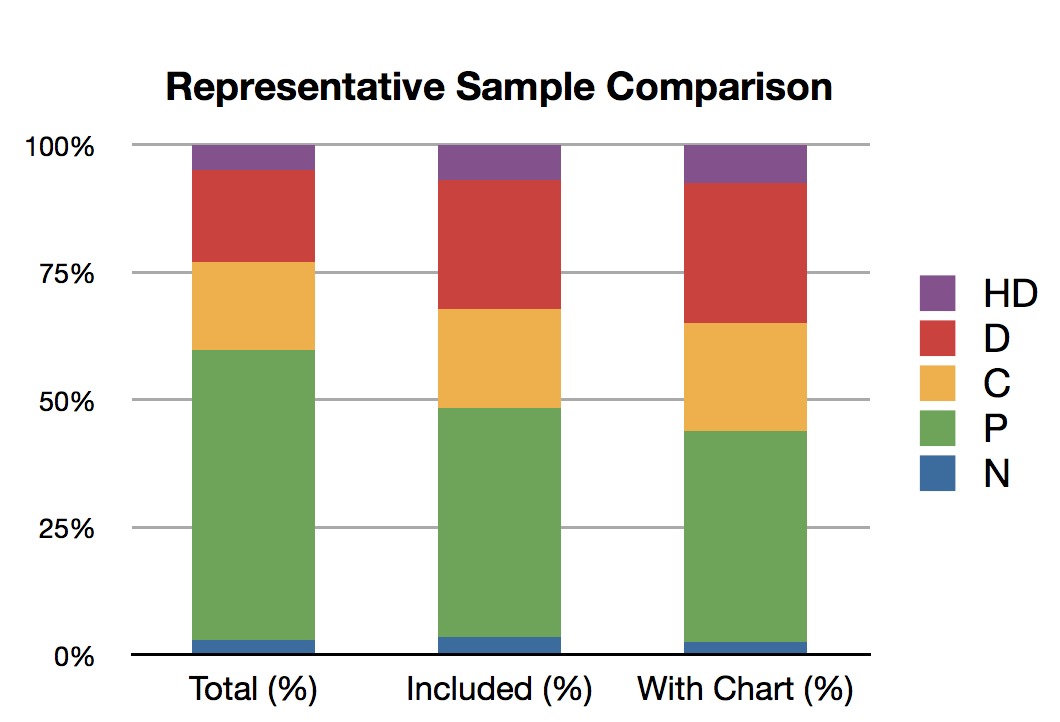
\includegraphics[width=0.7\textwidth]{ProgressGradeDistributions}
  \caption{Distribution of grades for the full unit, for those students who agreed to participate in the research, and those who included the burndown chart.}
  \label{fig:progress_grade_dist}
\end{figure}

% subsection sub:progress_student_cohort (end)

\subsubsection{Thematic Analysis to Identify Trends in Progress} % (fold)
\label{sub:approach_to_analysis}

The process from \sref{sub:thematic_analysis} was used in order to identify the themes and patterns associated with student progress. To gain familiarisation with the data, the burn down charts from each portfolio were scanned. Each page of the resulting document included the chart and a code to identify the portfolio from whence it came. To ease the process of visual classification the charts were scaled to similar size. Each chart was then printed and spread out in a large visual space to enable ``visual'' themes to be identified, and to determine appropriate classifications. 

Charts were classified based on the separation between the \textbf{Target Completion} line (target due dates), and the \textbf{Actual Completion} line, which indicated student progress based on the work having been signed off as complete by their Tutor. This process resulted in a number of chart classifications, and subclasses. Once the charts were classified they were examined again for any common features that occurred across classifications. 

% subsection approach_to_analysis (end)

\subsection{Results} % (fold)
\label{sec:progress_results}

\subsubsection{Identifed Chart Classifications} % (fold)
\label{sub:identified_chart_classifications}

Analysis of the charts made available to this research identified seven different classification related to the distance between the actual and target completion lines.Each classification is described in the following list, and illustrated in \tref{tbl:chart_types}.

% \begin{enumerate}[noitemsep,nolistsep]
%   \item Tight trend with little diversion from the target completion line (Class \textbf{A}).
%   \item Close to line and similar to Class A but with more deviation, though never more than one to two weeks delay before returning to the target completion line (Class \textbf{B}).
%   \item Consistently trending down, but with sustained small gap(s) from the target completion line (Class \textbf{C}).
%   \item Primarily off the target completion line, with occasional (rare) points where work caught up with the schedule (Class \textbf{D}). 
%   \item More distant from the line, but catching up toward the end of the unit (Class \textbf{E}).
%   \item Mostly distant from the line, with progress made in large steps (Class \textbf{F}).
%   \item Not complete, chart included but student was not able to get all work signed off (Class \textbf{N}).
% \end{enumerate}

\begin{table}[p]
  \centering
  \caption{Illustrations of the seven chart classifications identified in this work. The thinner blue line represents the Target Completion line, the thicker orange line the Actual Completion.}
  \label{tbl:chart_types}
  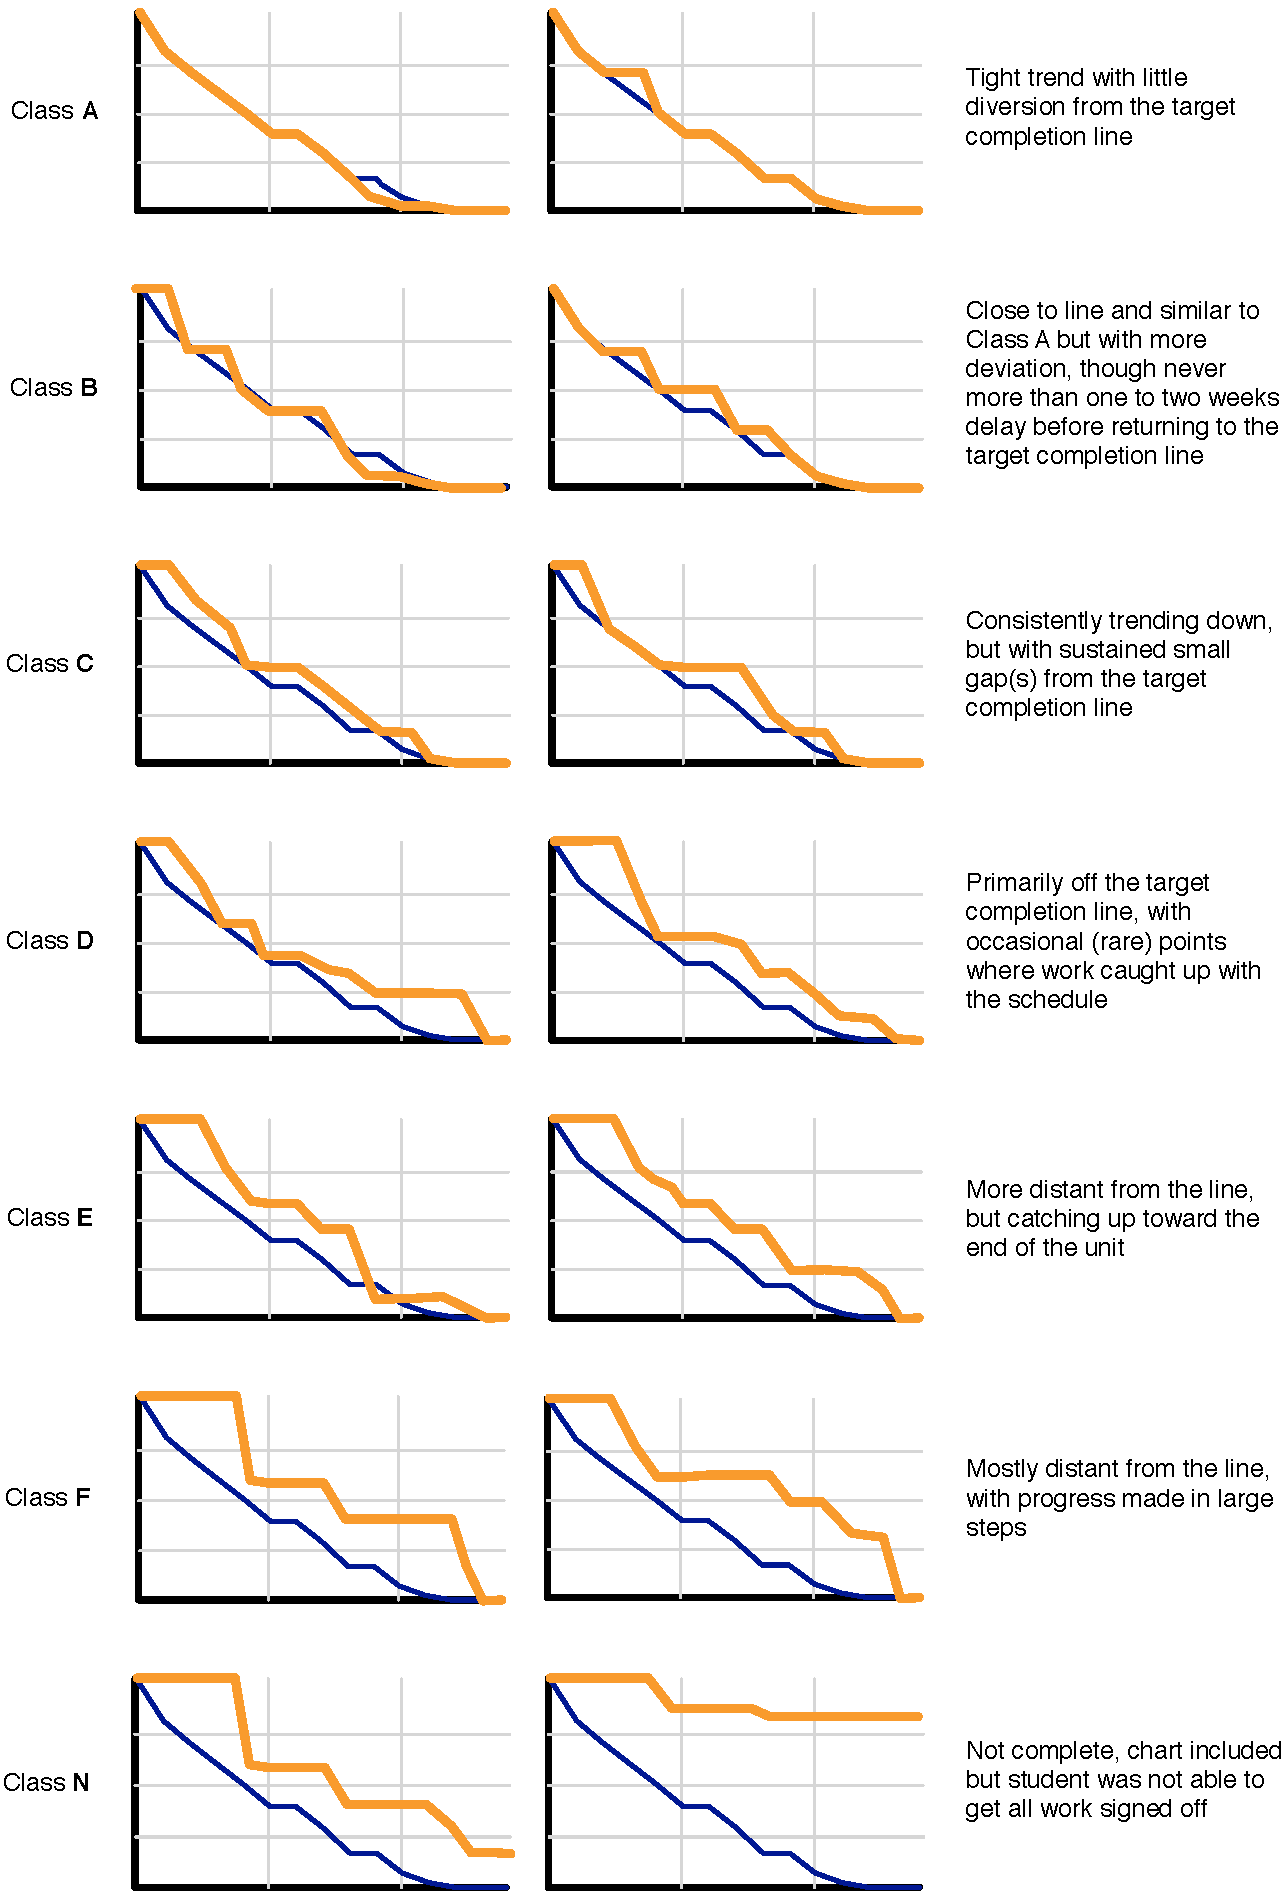
\includegraphics[width=\textwidth]{CharTypes}
\end{table}

\tref{tbl:chart_numbers} shows the frequency of each chart class in the analysed portfolios, and their associated grade distributions. The pie chart in \fref{fig:chart_dist} shows the distribution of the classifications, with the highlighted section indicating the number of students who did not get all tasks signed off (Class N).

\begin{table}[htbp]
  \footnotesize
  \renewcommand{\arraystretch}{1.3}
  \caption{Chart classification numbers, and grade distribution.}
  \label{tbl:chart_numbers}
  \centering
    \begin{tabular}{l|c|c|c|c|c|c}
        \textbf{Class} & \textbf{Total} & \textbf{HD} & \textbf{D} & \textbf{C} & \textbf{P}  & \textbf{N}  \\ \hline
        A     & 7     & 1  & 6 & 0 & 0  & 0  \\ 
        B     & 7     & 2  & 1 & 4 & 0  & 0  \\ 
        C     & 10    & 1  & 5 & 3 & 1  & 0  \\ 
        D     & 9     & 0  & 2 & 5 & 2  & 0  \\ 
        E     & 6     & 0  & 3 & 2 & 1  & 0  \\ 
        F     & 9     & 2  & 4 & 2 & 1  & 0  \\ 
        N     & 32    & 0  & 1 & 1 & 28 & 2  
    \end{tabular}
\end{table}

\begin{figure}[thb]
  \centering
  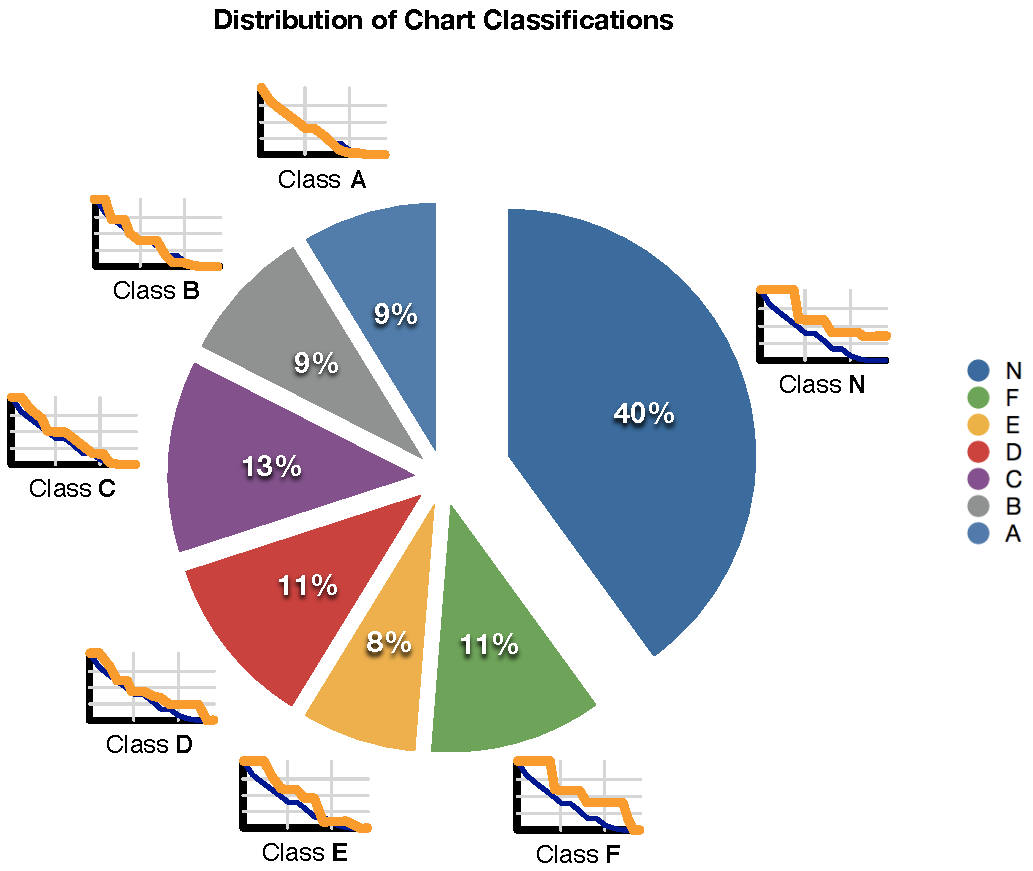
\includegraphics[width=0.8\textwidth]{DistributionOfChartClassifications}
  \caption{Distribution of portfolios according to chart class. Note that 40\% of students did not have all weekly tasks signed off.}
  \label{fig:chart_dist}
\end{figure}

% subsection primary_chart_categories (end)

\subsubsection{Chart Features and Subclasses} % (fold)
\label{sub:chart_subclasses}

% Most of the chart classifications presented a number of interesting features or identifiable subclasses.

Five of the seven Class A charts demonstrated cases where students got ahead of the scheduled work. This was also evident in five of the seven Class B charts, and three Class C charts. Of note are two students with Class D charts, more distant from the target completion line, who also managed to get ahead. A total of fifteen students were able to get ahead at some stage, and in all cases this occurred around week nine, after the shift to the C programming language. 

Two subclasses were evident in the Class C charts, as illustrated in \fref{fig:c_subclass}. The first subclass included a consistent gap from the scheduled line. This subclass constantly trended down, but did not rejoin the scheduled line during the semester. The second subclass exhibited a jagged shape with constant gaps coming back to the scheduled line at regular intervals. Interestingly none of the second subclass got ahead at any stage. Both subgroups consisted of five charts.

\begin{figure}[htbp]
  \centering
  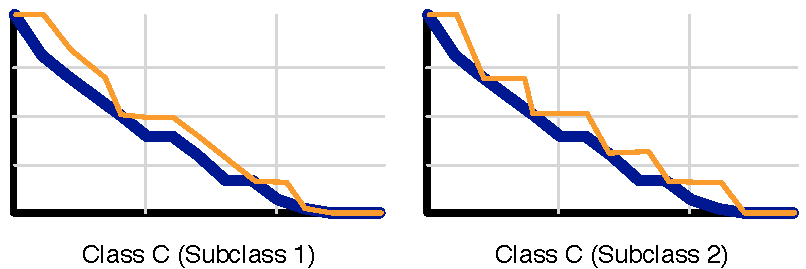
\includegraphics[width=0.8\textwidth]{ChartCSubclass}
  \caption{Illustrations of the two Class C subclasses, subclass 1 with a consistent gap and subclass 2 with a jagged sawtooth pattern.}
  \label{fig:c_subclass}
\end{figure}

The Class D charts had two identified subclasses, as illustrated in \fref{fig:d_subclass}. The larger subclass, subclass 1, had ``golf club'' shaped charts with effort at the end after a long period without progress (a flat line). The second subclass was characterised by a slow start, but catching up to the target completion line around the middle of the semester. The first subclass consisted of five charts, with four in the second subclass.

\begin{figure}[htbp]
  \centering
  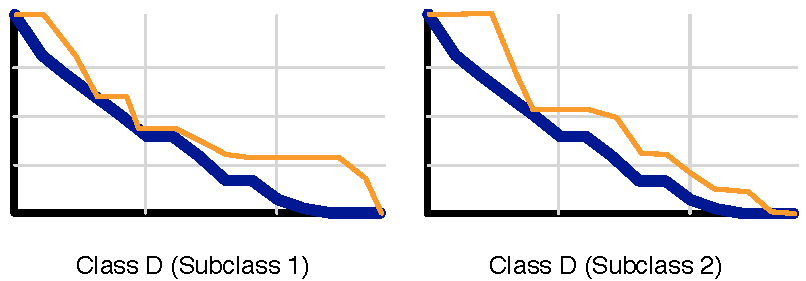
\includegraphics[width=0.8\textwidth]{ChartDSubclass}
  \caption{Illustrations of the two Class D subclasses, with the ``golf club'' shaped subclass 1.}
  \label{fig:d_subclass}
\end{figure}

\fref{fig:f_subclass} illustrates the three subclasses that were identified for the charts most distant from the scheduled line (Class F). The subclasses included (1) three large steps to reach the end, (2) a plateau mid semester then progress toward the end, and (3) a similar ``golf club'' shape to Class D with a large amount of work being signed off at the end of the semester. 

\begin{figure}[htbp]
  \centering
  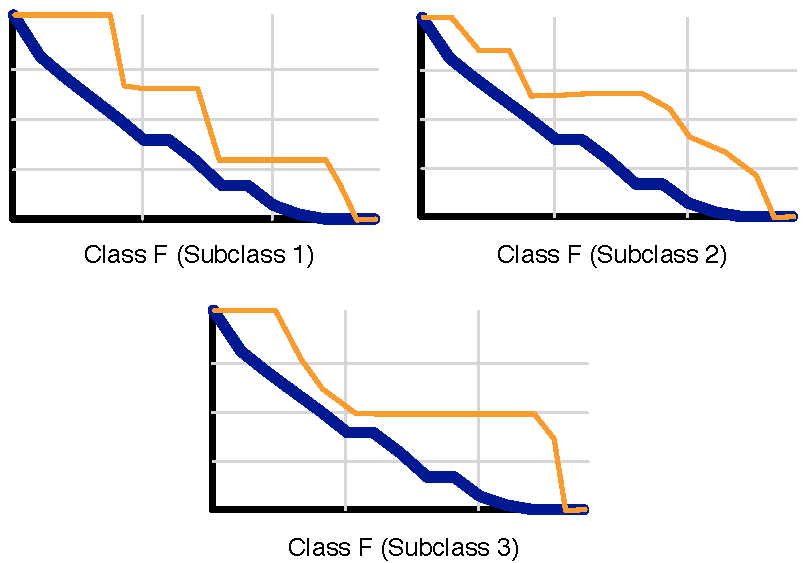
\includegraphics[width=0.8\textwidth]{ChartFSubclass}
  \caption{Illustrations of the three Class F subclasses, with three large steps for subclass 1, plateau in subclass 2, and larger ``golf club'' shape in subclass 3.}
  \label{fig:f_subclass}
\end{figure}

Of the 32 students who did not get all weekly tasks signed off (Class N) 13 (41\%) had completed 75\% or more of the work by the end of the unit. A further 9 had completed more than 50\%, 8 had more than 25\%, with 2 having less than 25\% of the work signed off. This is shown in visually in \fref{fig:n_subclass}, with the pie chart in \fref{fig:end_point} illustrating the percentage of each of the end points. Two portfolios in Class N were awarded grades higher than Pass as a result of special consideration.

\begin{figure}[htbp]
  \centering
  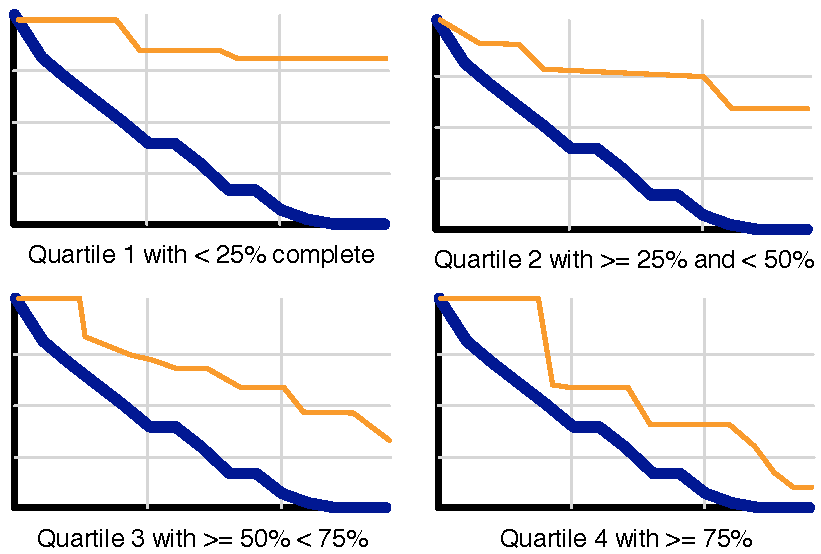
\includegraphics[width=0.8\textwidth]{ChartNSubclass}
  \caption{Illustrations of the different graph end points for Class N charts}
  \label{fig:n_subclass}
\end{figure}

\begin{figure}[thbp]
  \centering
  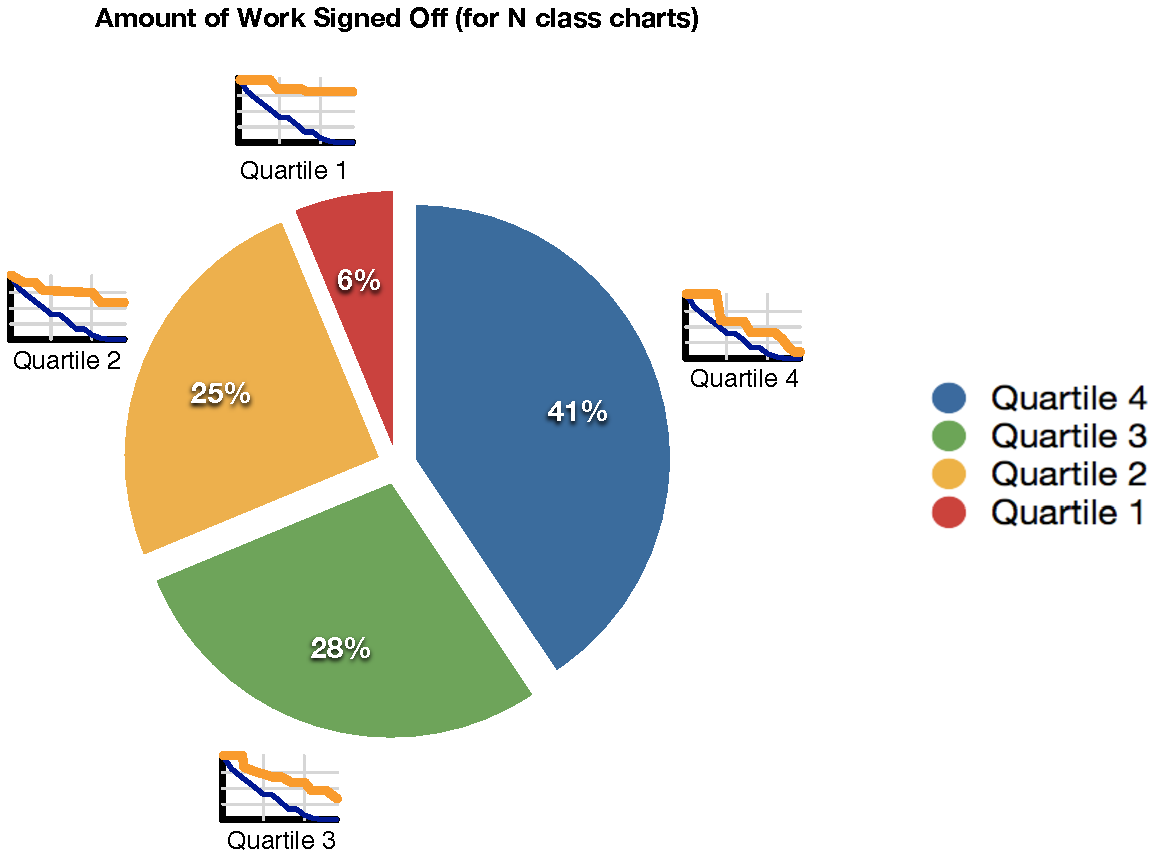
\includegraphics[width=0.9\columnwidth]{AmountSignedOffForN}
  \caption{Percentage tasks signed off for students with Class N charts.}
  \label{fig:end_point}
\end{figure}

Of the other classes, most charts that were close to the line (Class B) had their deviation around week five, which coincided with the arrays topic. Whereas the group more distant from the line (Class E) typically had slow starts with strong finishes. 

% subsection chart_subcategories (end)



\subsubsection{Grades by Chart Classification} % (fold)
\label{sub:grades_by_chart_classification}

\tref{tbl:chart_numbers} includes the result distribution for each chart class, shown graphically in \fref{fig:grade_chart_dist}. Pass results were primarily from Class N, Credit results were distributed across classes B through F, Distinction across classes A through F, with High Distinctions coming from classes A though C and F.

\begin{figure}[thb]
  \centering
  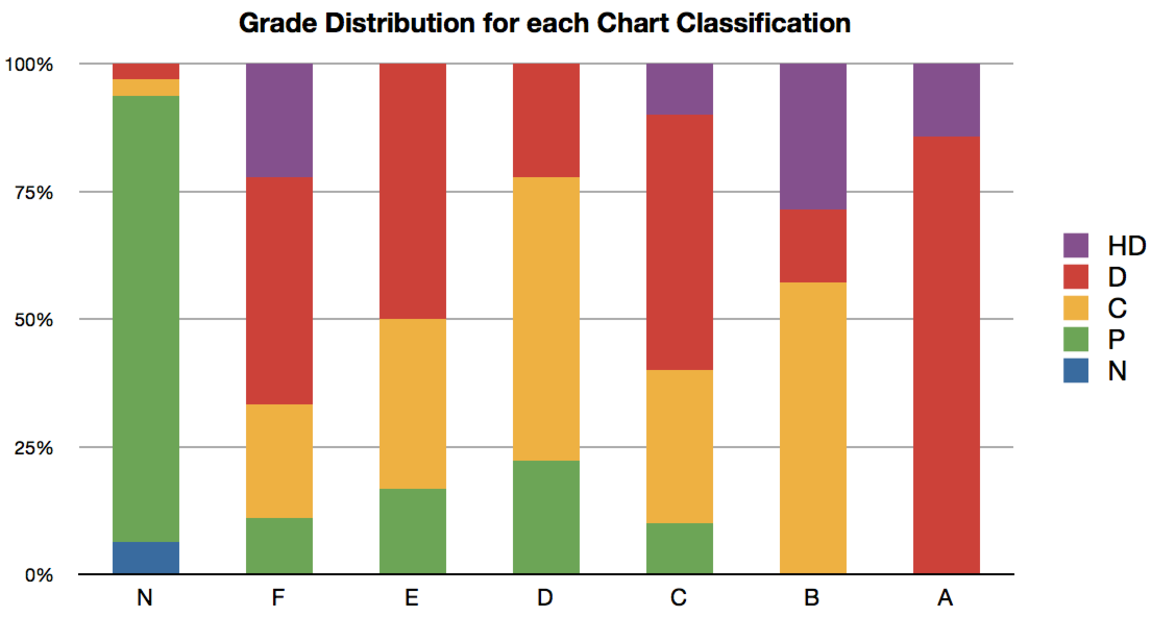
\includegraphics[width=0.8\columnwidth]{GradesForEachChartKind}
  \caption{Distribution of grades for each of the identified chart classes}
  \label{fig:grade_chart_dist}
\end{figure}


% subsection grades_by_chart_classification (end)


% section results (end)


\subsection{Discussion} % (fold)
\label{sec:progress_discussion}

\subsubsection{Focus of Investigation and Quality of Sample Used} % (fold)
\label{sub:focus_of_investigation_and_quality_of_sample_used}

% focus
Understanding how students progress through an introductory programming unit can provide valuable insight into the strategies they are using and the methodology underpinning the teaching and learning context. Our investigation examined burn down charts included in student portfolios, which captured the rate at which students were able to complete formative assessment tasks and have them signed off by their tutors.  Results of the visual thematic analysis, presented in Section \ref{sec:progress_results}, identified a number of different chart classes and presented details on associated result distributions.

% sample quality = good
The investigation examined a sample of the portfolios submitted in a single semester, with 80 (58\%) of the portfolios being included in the analysis. The distribution of grades for these groups are shown in \tref{tbl:progress_student_numbers} and \fref{fig:progress_grade_dist}. The relative distribution of grades in the group with charts is a reasonable representation of the entire unit, though the Pass grade is under represented. However, as the pass grade students tended to be clustered in Class N, it is likely that the sample captured the variations in general student progress across all grades.

% subsection focus_of_investigation_and_quality_of_sample_used (end)

\subsubsection{Participation in Formative Assessment} % (fold)
\label{sub:participation_in_formative_assessment}

A number of the charts indicate active student engagement with the formative assessment throughout the semester. This is evident in the chart classes A through C, D (subclass 2), E, and N (for those who completed between 75\% but less than 100\% of the scheduled tasks). This represented 47 (59\%) of the 80 charts, and in all cases the charts indicated ongoing progress, which was only possible by engaging with the formative process. 

Our interpretation of the charts from Class D Subclass 1, with its distinctive ``golf club'' shape, is that these students are likely to have their attention diverted mid-semester. A possible cause is that the due dates for first assignments in parallel, but unrelated, units typically fall in this period. Alternatively, these students may have needed additional time to bring all of the concepts together before continuing on with the C programming language. In either case, toward the end of the unit these students were then able to get back on track, and in some cases get ahead of schedule. It would be interesting for future work to examine the reflections of these students to verify these interpretations.

The large drops in the Class F charts may be evidence of confident students who only occasionally submit their work for assessment. This idea is supported by the large portion of D and HD results in this group.

A cause for concern is the large number of Class N charts, particularly where less than 75\% of the formative tasks were completed. This group made up 30 (38\%) of the 80 portfolios examined. The unit teaching staff indicated, overwhelmingly, that a lack of student engagement had been of particular concern for the semester under analysis. These students had little interest in learning to program, and seemed to have taken superficial approaches to learning and doing this work. This is evidenced in the both the final results and number of students with Class N charts.

% subsection participation_in_formative_assessment (end)


\subsubsection{Progress, Grades, and Formative Assessment} % (fold)
\label{sub:progress_grades_and_formative_assessment}

In reflecting on the distribution of grades across the different chart classifications, we believe that students have been able to achieve good results using a number of different strategies. If this is compared with units that use summative assessment during the semester, as illustrated in \fref{fig:pace}, students with charts in classes C through F are likely to have lost some marks early on, as they were behind the target completion line at various stages during the semester. With the portfolio approach, 50\% of these students were able to go on and achieve a Distinction or higher grade.

Of particular interest are the students with charts in class E, which was characterised by a slow start and a strong finish. These appear to be students who struggled with concepts initially but eventually gained sufficient mastery to quickly catch up later in the semester. It is interesting to note the large portion of these students who were subsequently able to achieve a Distinction result. Even with the slow start, these students were able to apply the concepts learnt to the creation of their own program. Had this been a traditional programming unit, using summative assessment during the semester, loss of marks early on  may have lead to them not receiving a grade that represented their final learning outcome. If these students lacked confidence, then this negative reinforcement may possibly discourage them from attempting to master the concepts, and reinforce any negative opinion they have of the field in general.

% subsection progress_grades_and_formative_assessment (end)

% B * Close to Line - also close matching but with slightly more deviation, but never more than one to two weeks delay. Those with a 2 week delay occurred around week 5 (arrays) - back on track at week 7. (4 of 7 - issues with arrays). Something has happened at this point, if this is related to content this may indicate issues with arrays in this group that then learned from their mistakes and were able to get back on track with sufficient feedback. - most of these dip under the line with the switch to C. (6 of 7)

\subsubsection{Concept Based Approach} % (fold)
\label{sub:use_of_multiple_languages}

The charts also provide evidence of the effectiveness of the concept-based approach used. A total of 15 (19\%) of the 80 charts showed students getting ahead of the schedule after the switch to the C programming language. This mostly consisted of students with charts in classes A and B, though it also includes several students in classes C and E. 

After the language change, tasks were concerned with expressing previously presented concepts in the C language. We propose that students who committed to understanding the underlying programming concepts, rather than focussing on the Pascal language itself, were able to exploit this understanding when introduced to C. Analysis of reflections in these portfolios may provide additional evidence to help verify this. 

% subsection use_of_multiple_languages (end)

\subsubsection{Reflecting on Programming Issues} % (fold)
\label{sub:relation_to_issues}

This work helps support two of the general learning issues, as identified in \sref{sec:issues_identified_in_student_reflections}, facing students: getting started, and learning through mistakes. Other than classes A and B, most of the student's progress appears to indicate that they had issues getting started. This is understandable, given the highly interrelated nature of the programming concepts presented in early weeks. The progress students showed later in the semester also demonstrates that students are able to make progress while learning through mistakes. 

In relation to time management -- the number one issue identified in our previous work -- further analysis of student reflections is needed to determine if the tool provided them with useful feedback and motivation to keep on track. That said, the tool was actively used and provided staff with useful information on student progress throughout the teaching period.

% subsection relation_to_issues (end)


% section discussion (end)

\subsection{Summary} % (fold)
\label{sec:progress_summary}

In this section we presented a visual thematic analysis of student progress as evidenced by burn down charts included in their final portfolios. Details of the unit, its delivery, assessment, and its use of burn down charts to track progress was described as a context for this work.  

Thematic analysis identified several different chart classes and subclasses, based on the shape of the chart and its distance from the target completion line. These classes provided some indication of students' approach to learning, with most concentrating on language features rather than underlying programming concepts. The different chart classes also presented evidence that students struggle to get started with introductory programming, but that once concepts were mastered they were able to catch up and, in some cases, get ahead of schedule. Interestingly, the use of formative feedback resulted in students being able to achieve high grades even when they struggled initially.

% section conclusion (end)

% chapter lessons_learnt_through_action_research (end)